\documentclass[
  bibliography=totoc,     % Literatur im Inhaltsverzeichnis
  captions=tableheading,  % Tabellenüberschriften
  titlepage=firstiscover, % Titelseite ist Deckblatt
]{scrartcl}

% Paket float verbessern
\usepackage{scrhack}

% Warnung, falls nochmal kompiliert werden muss
\usepackage[aux]{rerunfilecheck}

% unverzichtbare Mathe-Befehle
\usepackage{amsmath}
% viele Mathe-Symbole
\usepackage{amssymb}
% Erweiterungen für amsmath
\usepackage{mathtools}

% Fonteinstellungen
\usepackage{fontspec}
% Latin Modern Fonts werden automatisch geladen
% Alternativ zum Beispiel:
%\setromanfont{Libertinus Serif}
%\setsansfont{Libertinus Sans}
%\setmonofont{Libertinus Mono}

% Wenn man andere Schriftarten gesetzt hat,
% sollte man das Seiten-Layout neu berechnen lassen
\recalctypearea{}

% deutsche Spracheinstellungen
\usepackage[ngerman]{babel}


\usepackage[
  math-style=ISO,    % ┐
  bold-style=ISO,    % │
  sans-style=italic, % │ ISO-Standard folgen
  nabla=upright,     % │
  partial=upright,   % │
  mathrm=sym,        % ┘
  warnings-off={           % ┐
    mathtools-colon,       % │ unnötige Warnungen ausschalten
    mathtools-overbracket, % │
  },                       % ┘
]{unicode-math}

% traditionelle Fonts für Mathematik
\setmathfont{Latin Modern Math}
% Alternativ zum Beispiel:
%\setmathfont{Libertinus Math}

\setmathfont{XITS Math}[range={scr, bfscr}]
\setmathfont{XITS Math}[range={cal, bfcal}, StylisticSet=1]

% Zahlen und Einheiten
\usepackage[
  locale=DE,                   % deutsche Einstellungen
  separate-uncertainty=true,   % immer Unsicherheit mit \pm
  per-mode=symbol-or-fraction, % / in inline math, fraction in display math
]{siunitx}

% chemische Formeln
\usepackage[
  version=4,
  math-greek=default, % ┐ mit unicode-math zusammenarbeiten
  text-greek=default, % ┘
]{mhchem}

% richtige Anführungszeichen
\usepackage[autostyle]{csquotes}

% schöne Brüche im Text
\usepackage{xfrac}

% Standardplatzierung für Floats einstellen
\usepackage{float}
\floatplacement{figure}{htbp}
\floatplacement{table}{htbp}

% Floats innerhalb einer Section halten
\usepackage[
  section, % Floats innerhalb der Section halten
  below,   % unterhalb der Section aber auf der selben Seite ist ok
]{placeins}

% Seite drehen für breite Tabellen: landscape Umgebung
\usepackage{pdflscape}

% Captions schöner machen.
\usepackage[
  labelfont=bf,        % Tabelle x: Abbildung y: ist jetzt fett
  font=small,          % Schrift etwas kleiner als Dokument
  width=0.9\textwidth, % maximale Breite einer Caption schmaler
]{caption}
% subfigure, subtable, subref
\usepackage{subcaption}

% Grafiken können eingebunden werden
\usepackage{graphicx}

% schöne Tabellen
\usepackage{tabularray}
\UseTblrLibrary{booktabs, siunitx}

\DefTblrTemplate{contfoot-text}{normal}{Weiter auf der nächsten Seite}
\SetTblrTemplate{contfoot-text}{normal}
\DefTblrTemplate{conthead-text}{normal}{(Fortsetzung)}
\SetTblrTemplate{conthead-text}{normal}

% Verbesserungen am Schriftbild
\usepackage{microtype}

% Literaturverzeichnis
\usepackage[
  backend=biber,
]{biblatex}
% Quellendatenbank
\addbibresource{lit.bib}
\addbibresource{programme.bib}

% Hyperlinks im Dokument
\usepackage[
  german,
  unicode,        % Unicode in PDF-Attributen erlauben
  pdfusetitle,    % Titel, Autoren und Datum als PDF-Attribute
  pdfcreator={},  % ┐ PDF-Attribute säubern
  pdfproducer={}, % ┘
]{hyperref}
% erweiterte Bookmarks im PDF
\usepackage{bookmark}

% Trennung von Wörtern mit Strichen
\usepackage[shortcuts]{extdash}

\author{%
  Dominik Funcke\\%
  \href{mailto:dominik.funcke@tu-dortmund.de}{dominik.funcke@tu-dortmund.de}%
  \and%
  Pascal Machnik\\%
  \href{mailto:pascal.machnik@tu-dortmund.de}{pascal.machnik@tu-dortmund.de}%
}
\publishers{TU Dortmund – Fakultät Physik}

%Pakete zum definieren neuer commands
\usepackage{expl3}
\usepackage{xparse}

%mit \I kann man nun i aufrecht schreiben
\ExplSyntaxOn
\NewDocumentCommand \I {} {
  \symup{i}
}
\ExplSyntaxOff

%mit \E kann man nun e aufrecht schreiben
\ExplSyntaxOn
\NewDocumentCommand \E {} {
  \symup{e}
}
\ExplSyntaxOff

%mit \dif{x} kann man das d vor dem x aufrecht schreiben
\ExplSyntaxOn
\NewDocumentCommand \dif {m} {
  \mathinner{\symup{d} #1}
}
\ExplSyntaxOff
%mit \v kann man nun Vektoren schreiben
\ExplSyntaxOn
\let\vaccent=\v              % alten Befehl kopieren
\RenewDocumentCommand \v {}  % Befehl überschreiben
{
  \TextOrMath{
    \vaccent                  %Textmodus
  }{
  \symbf                      %Mathe modus
  } 
}
\ExplSyntaxOff

%besserer Real- und Imaginärteil
\AtBeginDocument{ % wird bei \begin{document} ausgeführt
  % werden sonst wieder von unicode-math überschrieben
  \RenewDocumentCommand \Re {} {\operatorname{Re}}
  \RenewDocumentCommand \Im {} {\operatorname{Im}}
}


%richtiges Spacing für klammern links und rechts
\usepackage{mleftright}

%mit \l und \r werden links und rechts die richtigen Abstaende bei den Klammern zum bsp. sinus gesetzt
\ExplSyntaxOn
\let\ltext=\l
\RenewDocumentCommand \l {}
{
  \TextOrMath{ \ltext }{ \mleft }
}
\let\raccent=\r
\RenewDocumentCommand \r {}
{
  \TextOrMath{ \raccent }{ \mright }
}
\ExplSyntaxOff

%mit \abs* wachsen Betragsstriche mit
\DeclarePairedDelimiter{\abs}{\lvert}{\rvert}
\DeclarePairedDelimiter{\norm}{\lVert}{\rVert}

%definierendes gleich
\newcommand{\defeq}{\vcentcolon=}
\newcommand{\eqdef}{=\vcentcolon}

%fuer mitwachsende klammern
\setlength{\delimitershortfall}{-1sp}

%deutsche long-table Umgebung
\DefTblrTemplate{contfoot-text}{normal}{Weiter auf der nächsten Seite}
\SetTblrTemplate{contfoot-text}{normal}
\DefTblrTemplate{conthead-text}{normal}{(Fortsetzung)}
\SetTblrTemplate{conthead-text}{normal}

%zum Zeichnen mit TikZ
%\RequirePackage{luatex85}
%\documentclass[margin=5pt]{standalone}
%\usepackage{tikz}
%\usepackage[
%  europeanresistors, % follow DIN
%  americaninductors, % foolow DIN, funny, isn't it?
%  siunitx,
%]{circuitikz}

\setlength{\parindent}{0pt} % no indent for paragraphs

\usepackage{wrapfig}

\usepackage{braket}

\subject{VERSUCH 51}
\title{Schaltungen mit Operationsverstärkern}
\date{%
  Durchführung: 14.04.2025
  \hspace{3em}
  Abgabe: 21.04.2025
}

\begin{document}

\maketitle
\thispagestyle{empty}
\tableofcontents
\newpage
\setcounter{page}{1}

\section{Zielsetzung}
\label{sec:Zielsetzung}
Ziel dieses Versuches ist es, die Funktionsweise von Operationsverstärkern zu verstehen
und deren Eigenschaften zu untersuchen. Dazu werden verschiedene Schaltungen mit Operationsverstärkern
aufgebaut und deren Verhalten analysiert.
\section{Theorie}
\label{sec:Theorie}

In diesem Abschnitt soll die Funktionsweise des Operationsverstärkers (Op-Amp) und dessen Implementierung
in verschiedenen Schaltungen erklärt werden.

\subsection{Der Operationsverstärker}
\label{sec:Operationsverstaerker}
Der Operationsverstärker (Op-Amp) ist ein elektronisches Bauelement, das als Verstärker
der Differenzspannung zwischen zwei Eingängen fungiert. Ein Schaltbild eines Op-Amps ist in
\autoref{fig:opamp} dargestellt. 

\begin{figure}
    \centering
    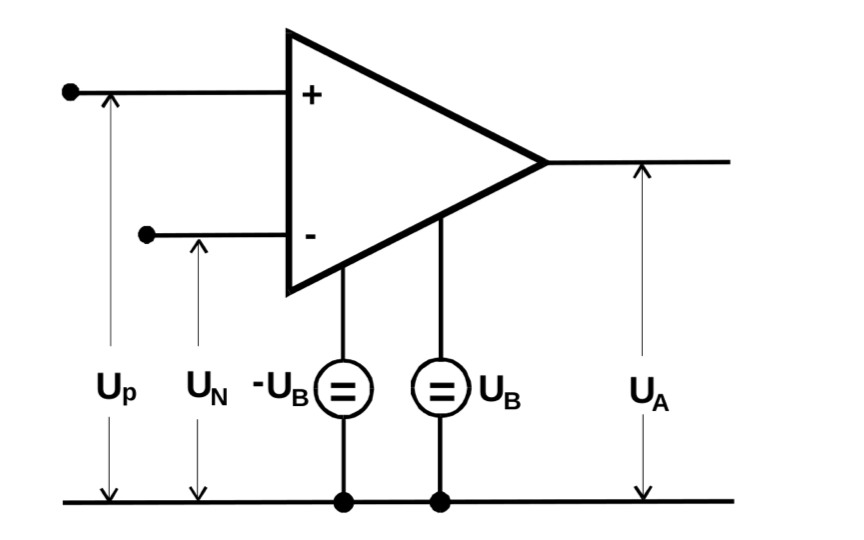
\includegraphics[width =0.48\textwidth]{figures/op-amp.png}
    \caption{Schaltbild eines Operationsverstärkers \cite{OP-Amp}.}
    \label{fig:opamp}
\end{figure}

Der Op-Amp hat zwei Eingänge, den nicht-invertierenden Eingang
($+$) und den invertierenden Eingang ($-$). Die Ausgangsspannung $U_\text{A}$ ist

\begin{equation}
    U_\text{A} = A \, (U_+ - U_-)
    \label{eq:OpAmp}
\end{equation}

mit $A$ als frequenzunabhängige Leerlaufverstärkung des Op-Amps. Die Spannungsversorgung findet über zwei 
Stromversorgungsanschlüsse statt, die hier mit $+U_\text{B}$ bzw. $-U_\text{B}$ bezeichnet sind. Diese definieren
den Bereich der Ausgangsspannung

\begin{equation}
    -U_{\text{B}} < U_{\text{A}} < U_{\text{B}}.
\end{equation}

\subsection{Der ideale Operationsverstärker}
\label{sec:IdealerOperationsverstaerker}
Der ideale Operationsverstärker ist ein theoretisches Modell, das einige Annahmen über den
Op-Amp trifft, um seine Eigenschaften zu vereinfachen. Diese Annahmen sind:
\newpage
\begin{itemize}
    \item Unendliche Leerlaufverstärkung $A \to \infty$.
    \item Unendlicher Eingangsimpedanz $Z_\text{e} \to \infty$.
    \item Null Ausgangsimpedanz $Z_\text{a} = 0$.
    \item Unendliche Bandbreite.
    \item Null Offsetspannung.
\end{itemize}

In der Praxis sind diese Annahmen nicht erfüllt, jedoch näherungsweise gültig, weshalb für die folgenden
Betrachtungen die Eigenschaften des ideale Operationsverstärker angenommen werden.

\subsection{Verschiedene Schaltungen mit Operationsverstärkern}
\label{sec:OperationsverstaerkerSchaltungen}
In diesem Abschnitt werden verschiedene Schaltungen mit Operationsverstärkern vorgestellt, welche in diesem
Versuch untersucht werden.

\subsubsection{Invertierender Verstärker}
\label{sec:InvertierenderVerstaerker}
Das Schaltbild eines invertierenden Verstärkers ist in \autoref{fig:invertierenderVerstaerker} 
dargestellt.

\begin{figure}
    \centering
    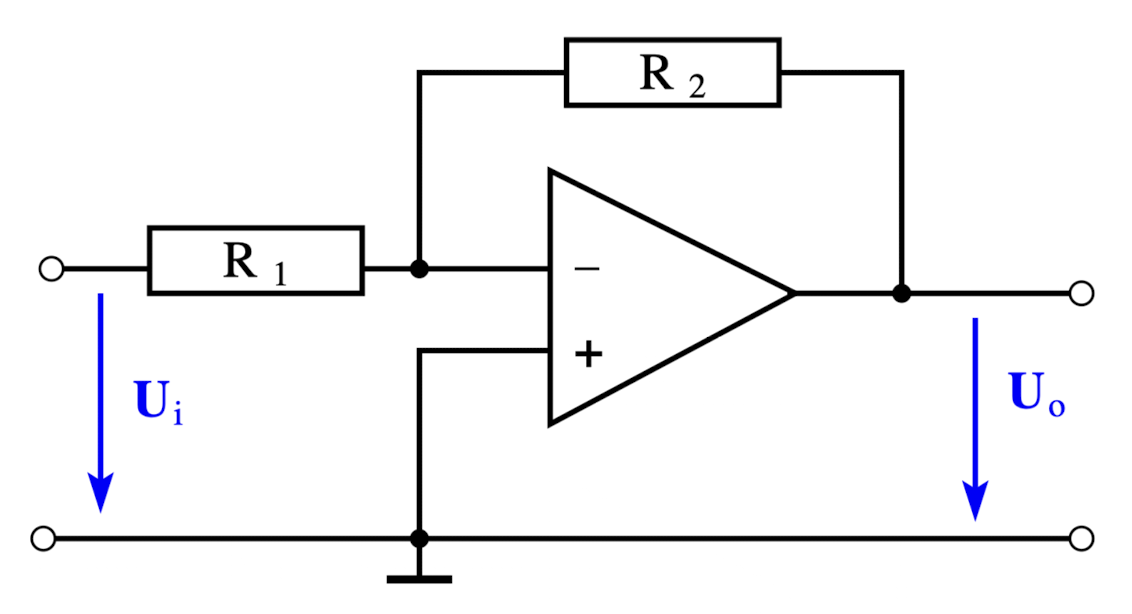
\includegraphics[width =0.48\textwidth]{figures/invertierender_verstärker.png}
    \caption{Schaltbild eines invertierenden Verstärkers \cite{Versuchsanleitung}.}
    \label{fig:invertierenderVerstaerker}
\end{figure}

Hierbei ist der nicht invertierende Eingang geerdet und der invertierende Eingang über eine Rückkopplung mit 
mit einem Widerstand mit dem Ausgang verbunden, sodass die Differenzspannung zwischen den Eingängen 
des OP-Amps verschwindet. Da das Eingangssignal $U_\text{i}$ an den invertierenden Eingang des Op-Amps 
angeschlossen ist, wird das Ausgangssignal $U_\text{o}$ invertiert. Dabei ist die Verstärkung des 
invertierenden Verstärkers durch das Verhältnis der Widerstände $R_1$ und $R_2$ gegeben

\begin{equation}
    U_\text{o} = - \frac{R_2}{R_1} \cdot U_\text{i}.
    \label{eq:invertierenderVerstaerker}
\end{equation}

\subsubsection{Integrator}
\label{sec:Integrator}
Das Schaltbild eines Integrators ist in \autoref{fig:integrator} 
dargestellt.

\begin{figure}[H]
    \centering
    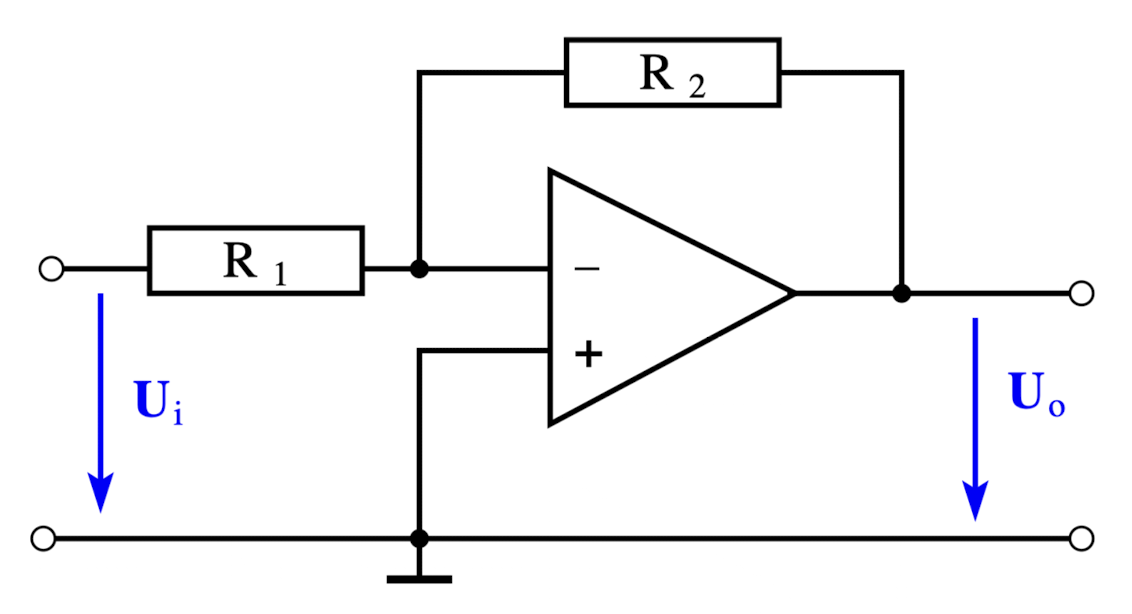
\includegraphics[width =0.48\textwidth]{figures/integrator.png}
    \caption{Schaltbild eines Integrators \cite{Versuchsanleitung}.}
    \label{fig:integrator}
\end{figure}

Hierbei ist der nicht invertierende Eingang geerdet und der invertierende Eingang über eine Rückkopplung
mit einem Kondesator mit dem Ausgang verbunden, sodass die Differenzspannung zwischen den Eingängen
des OP-Amps verschwindet. Das Ausgangssignal ist hierbei gegeben als

\begin{equation}
    U_\text{o} = - \frac{1}{R C} \, \int U_\text{i} \, \dif{t}.
    \label{eq:integrator}
\end{equation}

Angenommen ein Sinussignal $U_{\text{i}} = A \sin(2 \pi f)$ mit der Frequenz $f$ wird an den Eingang des 
Integrators angelegt, so ergibt sich als Ausgangssignal 

\begin{equation}
    U_\text{o} = - \frac{A}{2 \pi R C f} \, \cos(2 \pi f) \propto \frac{1}{f}.
    \label{eq:integratorSinus}
\end{equation}

\subsubsection{Differenzierer}
\label{sec:Differenzierer} 
Das Schaltbild eines Differenzierers ist in \autoref{fig:differenzierer}
dargestellt.

\begin{figure}
    \centering
    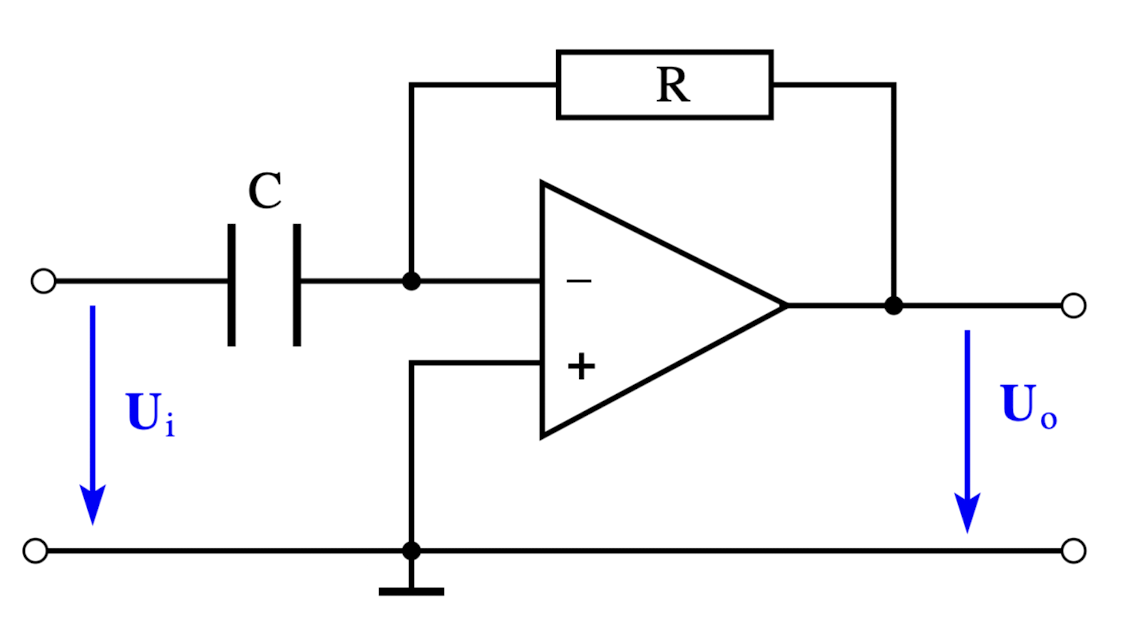
\includegraphics[width =0.48\textwidth]{figures/differenzierer.png}
    \caption{Schaltbild eines Differenzierers \cite{Versuchsanleitung}.}
    \label{fig:differenzierer}
\end{figure}

Hierbei ist der nicht invertierende Eingang geerdet und der invertierende Eingang über eine Rückkopplung
mit einem Widerstand mit dem Ausgang verbunden, sodass die Differenzspannung zwischen den Eingängen
verschwindet. Vor dem invertierenden Eingang ist ein Kondensator geschaltet. Dieser Aufbau führt dazu,
dass das Ausgangssignal $U_\text{o}$ proportional zur Ableitung des Eingangssignals $U_\text{i}$ ist

\begin{equation}
    U_\text{o} = - R C \, \frac{\dif{U_\text{i}}}{\dif{t}}.
    \label{eq:differenzierer}
\end{equation}

Angenommen ein Sinussignal $U_{\text{i}} = A \sin(2 \pi f)$ mit der Frequenz $f$ wird an den Eingang des
Differenzierers angelegt, so ergibt sich als Ausgangssignal

\begin{equation}
    U_\text{o} = - 2 A R C \pi f \, \cos(2 \pi f) \propto f.
    \label{eq:differenziererSinus}
\end{equation}

\subsubsection{Schmitt Trigger}
\label{sec:SchmittTrigger}
Das Schaltbild eines Schmitt Triggers ist in \autoref{fig:schmittTrigger}
dargestellt.

\begin{figure}[H]
    \centering
    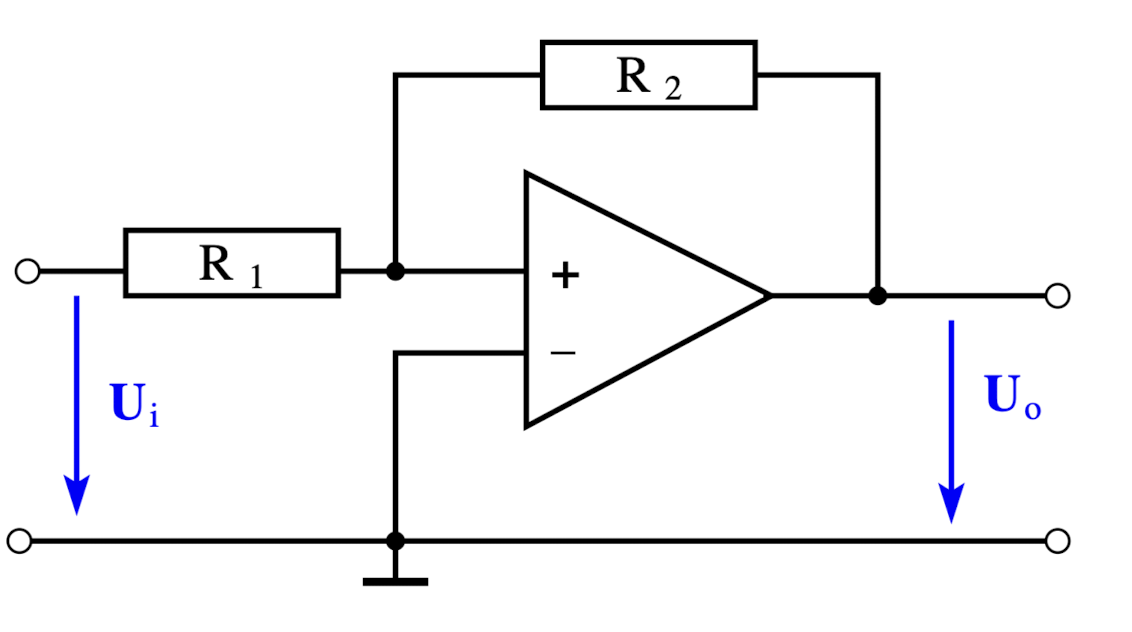
\includegraphics[width =0.48\textwidth]{figures/schmitt_trigger.png}
    \caption{Schaltbild eines Schmitt Triggers \cite{Versuchsanleitung}.}
    \label{fig:schmittTrigger}
\end{figure}

Im wesentlichen ist der Aufbau analog zum invertierenden Verstärker, jedoch findet die Rückkopplung zum
nicht invertierenden Eingang statt. Dadurch wird eine Hysterese erzeugt, die in \autoref{fig:schmittTriggerHysterese}
zu sehen ist.

\begin{figure}[H]
    \centering
    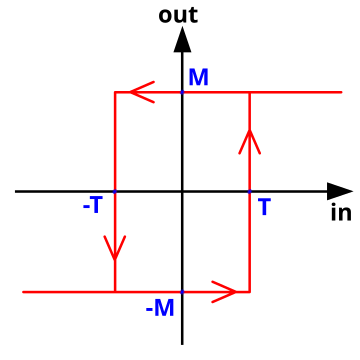
\includegraphics[width =0.48\textwidth]{figures/hysterese.png}
    \caption{Hysterese des Schmitt Triggers \cite{Schmitt-Trigger}.}
    \label{fig:schmittTriggerHysterese}
\end{figure}

Dabei ist die obere bzw. untere Schaltschwelle $\pm T$ gegeben durch

\begin{equation}
    T = \frac{R_2}{R_1} \, U_\text{B}.
    \label{eq:SchmittTriggerSchaltschwelle}
\end{equation}

Die Ausgangsspannung $U_\text{o}$ ist hierbei gegeben durch

\begin{equation}
    U_\text{o} = \begin{cases}
        U_\text{B} & \text{für } U_\text{i} > T \\
        -U_\text{B} & \text{für } U_\text{i} < -T
    \end{cases}.
\end{equation}

In allen anderen Fällen verbleibt der Schmitt Trigger in seinem aktuellen Zustand.

\subsubsection{Generator}
Das Schaltbild eines Generators ist in \autoref{fig:generator}
dargestellt.

\begin{figure}[H]
    \centering
    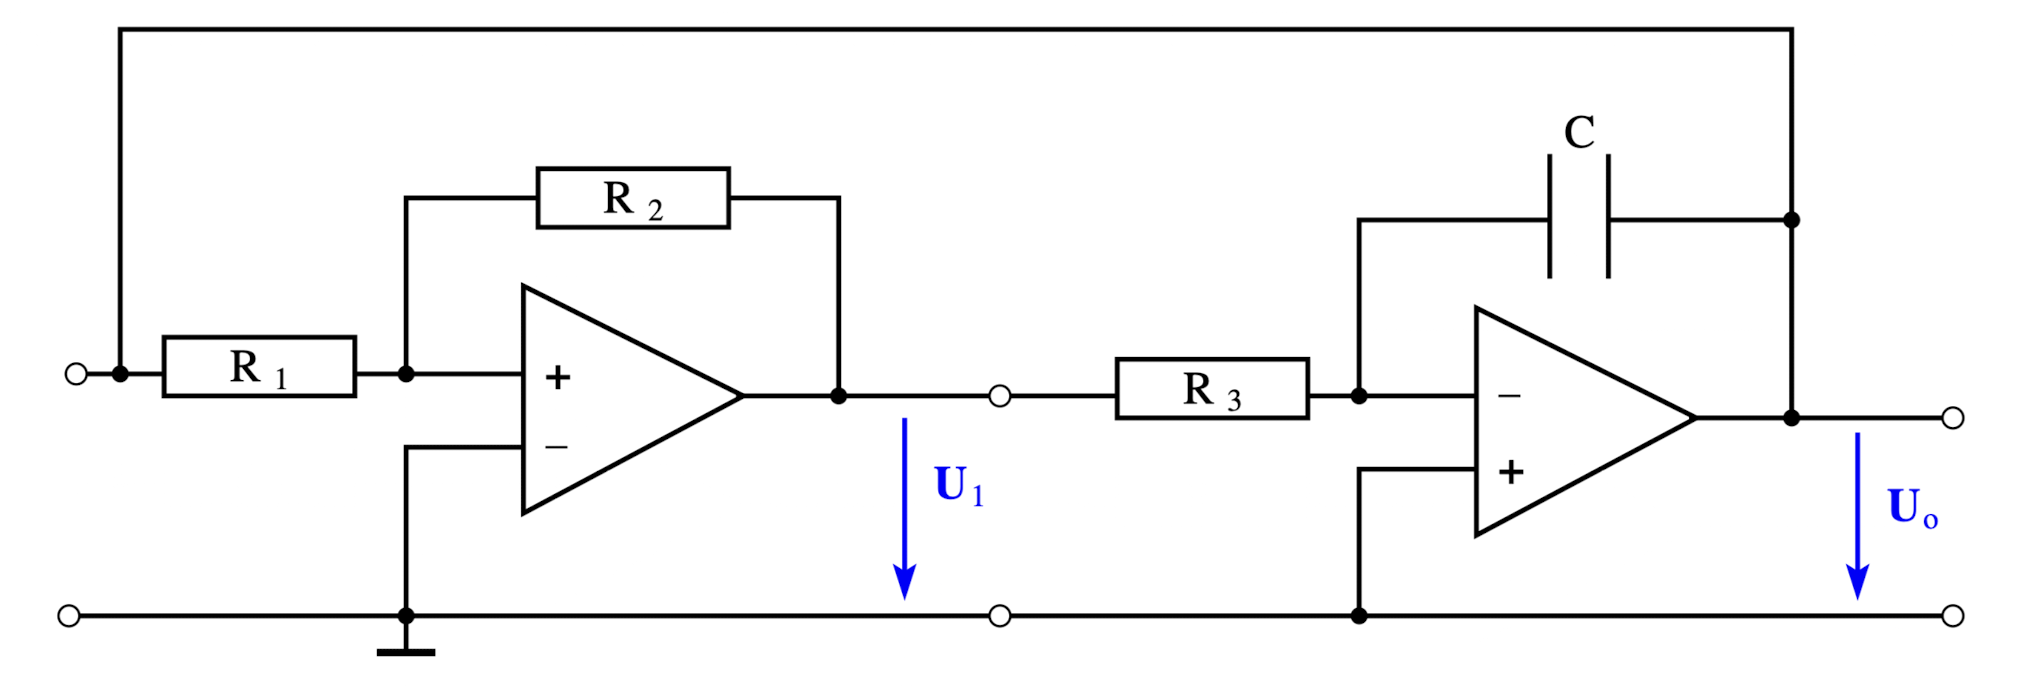
\includegraphics[width =0.8\textwidth]{figures/generator.png}
    \caption{Schaltbild eines Generators \cite{Versuchsanleitung}.}
    \label{fig:generator}
\end{figure}

Hierbei werden ein Schmitt Trigger und ein Integrator in Reihe geschaltet. Wobei der Output des
Integrators mit dem Eingang des Schmitt Triggers verbunden ist.
Durch diese Anordnung wird ein Rechtecksignal am Schmitt Trigger und ein Dreickssignal am 
Integrator mit der Frequenz 

\begin{equation}
    f = \frac{R_2}{4 C R_1 R_3}.
    \label{eq:GeneratorFrequenz}
\end{equation}

erzeugt, dessen Amplitude $A$ gegeben ist durch

\begin{equation}
    A = \frac{R_1}{R_2} \, U_\text{B}.
    \label{eq:GeneratorAmplitude}
\end{equation}

\subsubsection{Generator mit variierender Amplitude}
\label{sec:GeneratorMitVariierenderFrequenz}
Das Schaltbild eines Generators mit variierender Amplitude ist in \autoref{fig:generatorMitVariierenderAmplitude}
dargestellt.

\begin{figure}[H]
    \centering
    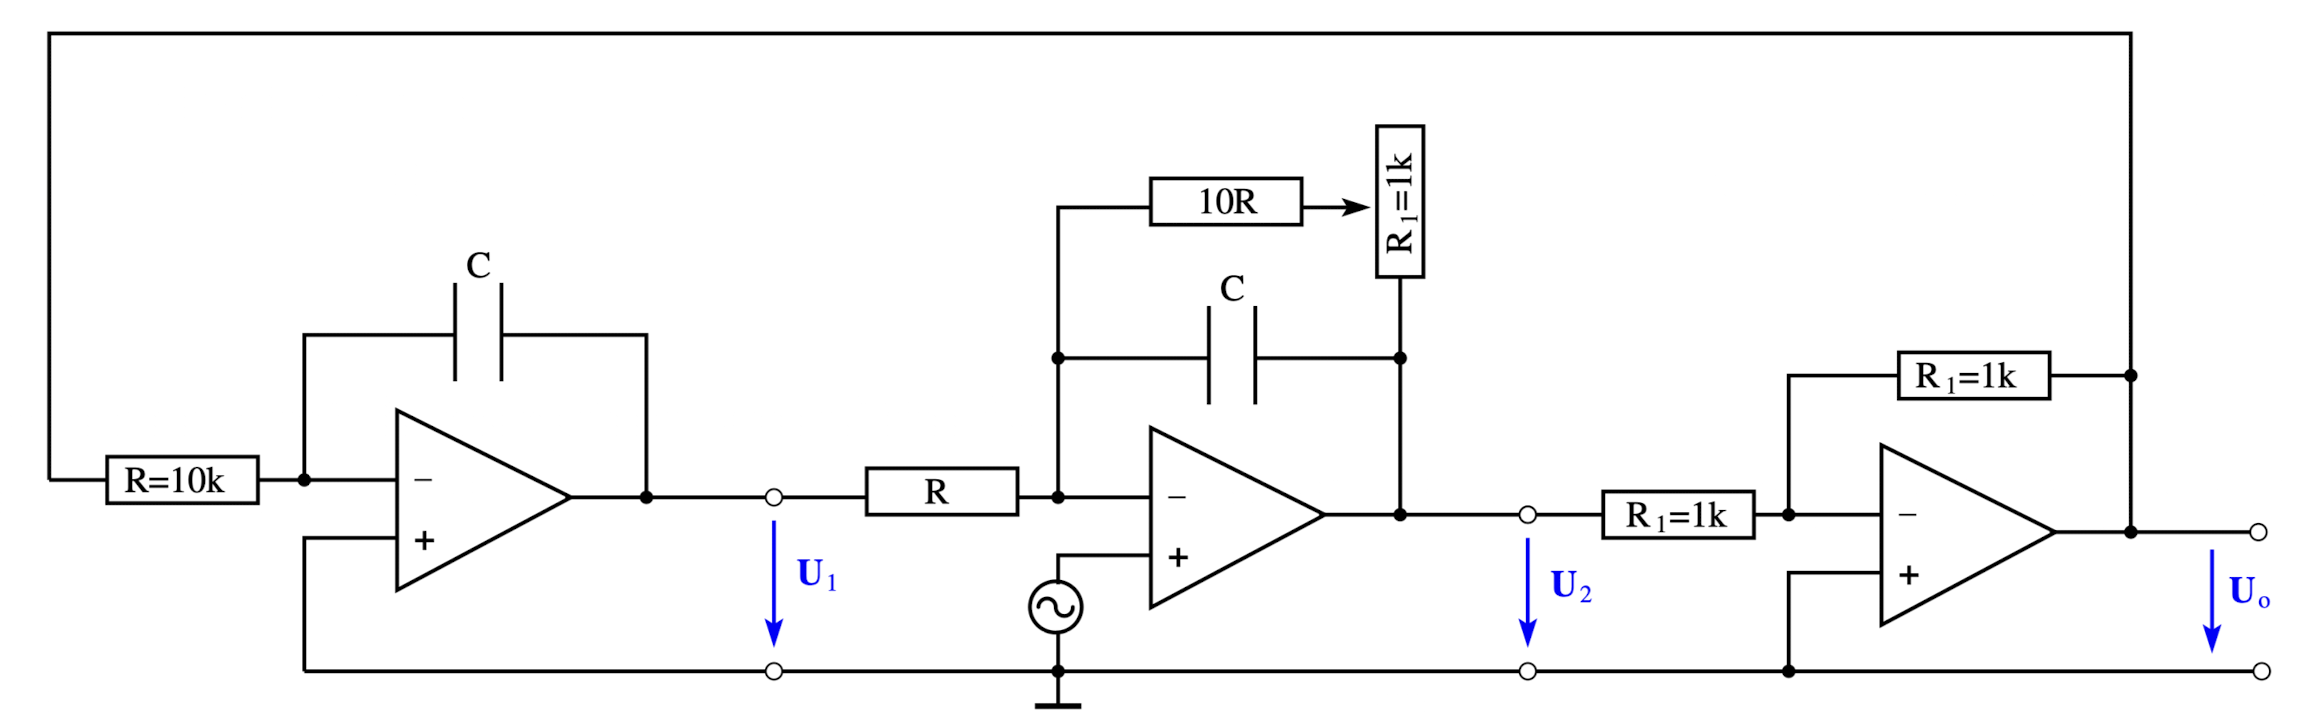
\includegraphics[width =0.8\textwidth]{figures/generator_mit_variierender_frequenz.png}
    \caption{Schaltbild eines Generators mit variierender Frequenz \cite{Versuchsanleitung}.}
    \label{fig:generatorMitVariierenderAmplitude}
\end{figure}

Es werden dafür zwei Integratoren und ein invertierender Verstärker in Reihe geschaltet. Dies führt 
dazu, dass eine gedämpfte harmonische Schwingung erzeugt wird, die durch die DGL 

\begin{equation}
    \frac{\symup{d}^2 U_\text{o}}{\dif{t^2}} - \frac{\eta}{10 RC} \, \frac{\dif{U_{\text{o}}}}{\dif{t}} + \frac{1}{R^2 C^2} \, U_{\text{o}} = 0
\end{equation}

beschrieben wird. Dabei ist $-1 \le \eta \le 1$ die Dämpfungskonstante, welche durch das Potentiometer eingestellt werden kann.
Die Lösung dieser DGL, unter der Annahme $\eta \ll 100$, ist gegeben durch

\begin{equation}
    U_\text{o}(t) = A \, \exp \l(-\frac{t}{\tau}\r) \, \sin \l(2 \pi \frac{t}{T}\r)
    \label{eq:GeneratorMitVariierenderAmplitudeLoesung}
\end{equation}

mit der Schwingungsdauer $T$ und der Zeitkonstante $\tau$, welche gegeben sind durch

\begin{equation}
    T = 2 \pi RC \quad \text{und} \quad \tau = \frac{20 RC}{\eta}.
    \label{eq:generatorMitVariierenderAmplitude}
\end{equation}
%\subsection{Berechnung der Messunsicherheiten}
\label{sec:Messunsicherheiten}

Zur Berechnung des Mittelwertes einer Größe $x$ mit $N$ Messwerten wird die Formel
%
\begin{equation}
    \bar{x} = \frac{1}{N} \sum_{i=1}^N x_i
\end{equation}
%
benutzt. Die zugehörige Standardabweichung des Mittelwertes $\increment \bar{x}$ berechnet sich über
%
\begin{equation}
    \increment \bar{x} = \sqrt{\frac{1}{N \l(N-1\r)}\sum_{i=1}^N \left(x_i - \bar{x}\right)^2}
\end{equation}
%
Die Unsicherheit einer zusammengesetzen Größe $g\left(x_1, …, x_n\right)$ wird mithilfe der Gaußschen
Fehlerfortpflanzung bestimmt
%
\begin{equation}
    \increment g\left(x_1, …, x_n\right) = \sqrt{\sum_{i=1}^N \left(\increment x_i ~ \partial_i \, f \right)^2}
\end{equation}
%
Größen werden in der Form $\bar{x} \pm \increment \bar{x}$ angegeben. Alle Berechnungen, Graphen, sowie die 
Bestimmung der Messunsicherheiten werden mit Python 3.11.5 und entsprechenden Bibliotheken
\footnote{Numpy \cite{numpy}, Matplotlib \cite{matplotlib} und Uncertainties \cite{uncertainties}} durchgeführt.
\section{Versuchsaufbau und Durchführung}
\label{sec:Durchführung}

\subsection{Invertierender Verstärker}
\label{subsec:InvertierenderVerstaerker}
Zur Untersuchung des Frequenzverhaltens eines invertierenden Verstärkers wird die Schaltung gemäß \autoref{fig:invertierenderVerstaerker} 
auf einem Steckbrett realisiert. Als Operationsverstärker wird ein 8pin LM741 Chip verwendet.
Zunächst werden die Widerstände auf $R_1 = \qty{1}{\kilo\ohm}$ und $R_2 = \qty{100}{\kilo\ohm}$ gesetzt, was einer erwarteten Verstärkung von 
$-R_2/R_1 = -100$ entspricht. 
Mit einem Funktionsgenerator wird eine sinusförmige Eingangsspannung mit konstanter Amplitude 
$U_\text{in} = \qty{300}{\milli\volt}$ über einen Frequenzbereich von $\qty{1}{\hertz}$ bis $\qty{100}{\kilo\hertz}$ eingespeist.
Für jede Frequenz wurde die Ausgangsspannung $U_\text{out}$ gemessen.
Zur Untersuchung des Verstärkungsverhaltens bei unterschiedlichen Parametern wird die Messung anschließend mit den Parametern 
$(R_1 = \qty{1}{\kilo\ohm}, R_2 = \qty{150}{\kilo\ohm}, U_\text{in} = \qty{100}{\milli\volt})$ und 
$(R_1 = \qty{1}{\kilo\ohm}, R_2 = \qty{10}{\kilo\ohm}, U_\text{in} = \qty{100}{\milli\volt})$ wiederholt.
Die Messdaten werden für jede Konfiguration in doppelt-logarithmischen Bode-Diagrammen dargestellt. Dabei wurde der Frequenzverlauf der 
Verstärkung analysiert und mithilfe eines Fits eine charakteristische Verstärkung, die Grenzfrequenz und die Bandbreite bestimmt.

\subsection{Integrator}
\label{subsec:Integrator}
Das Verhalten eines Integrators, gemäß der Schaltung in \autoref{fig:integrator},
wird - analog zum invertierenden Verstärker - mithilfe eines Steckbretts aufgebaut. Der Widerstand wird auf $R = \qty{10}{\kilo\ohm}$
und die Kapazität auf $C = \qty{22}{\nano\farad}$ festgelegt. Eine sinusförmige Eingangsspannung mit konstanter Amplitude
$U_\text{in} = \qty{1}{\volt}$ wird in den Schaltkreis eingespeist, und die Wertepaare $(U_\text{out}, f)$ werden aufgenommen.
Anschließend wird der Schaltkreis qualitativ auf seine Funktionsweise geprüft, indem ein Dreieck- sowie ein Rechtecksignal angelegt werden.
Die Displayanzeige des Oszilloskops wird jeweils als PNG-Datei gespeichert, und die Abbildungen in der Diskussion~\ref{sec:Diskussion}
auf das erwartete Verhalten hin analysiert. Die verwendete Frequenz und Eingangsspannung werden dabei so angepasst,
dass ein möglichst klares Bild auf dem Oszilloskop zu erkennen ist. Die genauen Parameter sind jeweils in den Abbildungen ersichtlich.

\subsection{Differenzierer}
\label{subsec:Differenzierer}
Das Verhalten einer Differenzierers wird genau Analog zum \autoref{subsec:Integrator} des Integrators analysiert.
Es werden jedoch die Parameter $R = \qty{100}{\kilo\ohm}$, $ C = \qty{22}{\nano\farad}$ und $V_{\text{in}} = \qty{90}{\milli\volt}$ verwendet.

\subsection{Schmitt Trigger}
\label{subsec:SchmittTrigger}
Die Schaltskizze in \autoref{fig:schmittTrigger} eines Schmitt-Triggers wird mithilfe von zwei 8-Pin-LM741-Chips
auf dem Steckbrett realisiert. Die verwendeten Parameter lauten $R_1 = \qty{10}{\kilo\ohm}$ und $R_2 = \qty{100}{\kilo\ohm}$.
Außerdem wird eine sinusförmige Signalspannung mit der Frequenz $\qty{1}{\kilo\hertz}$ verwendet.
Die Eingangsspannung wird zunächst auf $\qty{0}{\volt}$ gesetzt und anschließend schrittweise erhöht,
bis das Ausgangssignal gerade auf den High-Pegel umspringt.
Die zugehörigen Werte für $V_\text{in}$ und $V_\text{out}$ werden notiert.

\subsection{Generator}
\label{subsec:Generator}
Ein Generator gemäß \autoref{fig:generator} wird mit den Parametern 
$R_1 = \qty{10}{\kilo\ohm}$, $R_2 = \qty{100}{\kilo\ohm}$, $R_3 = \qty{1}{\kilo\ohm}$ und $C = \qty{1}{\micro\farad}$ betrieben. 
Das System sollte beim Einschalten der Spannungsversorgung für die 8-Pin-LM741-Chips anfangen zu oszillieren,
dies kann jedoch durch mehrfaches Ein- und Ausschalten der Stromversorgung unterstützt werden. 
Das Bild, das auf dem Display des Oszilloskops sichtbar ist und die Spannungen $U_o$ und $U_1$ aus \ref{fig:generator} zeigt, 
wird als PNG-Datei gespeichert.

\subsection{Generator mit variierenden Amplituden}
\label{subsec:GeneratorMitVariierendenAmplituden}
Mit den Widerständen $R = \qty{10}{\kilo\ohm}$, $R_1 = \qty{1}{\kilo\ohm}$, einem Widerstand $10R$, einem Potenziometer mit bis zu $\qty{1}{\kilo\ohm}$, 
einem Kondensator mit einer Kapazität von $C = \qty{100}{\nano\farad}$ und einem Funktionsgenerator, welcher hier eine rechteckige Spannung produziert, 
wird der Aufbau aus \autoref{fig:generatorMitVariierenderAmplitude} reproduziert.
Die Messdaten des Oszilloskops werden als CSV-Datei gespeichert und zusätzlich wird eine PNG-Datei des Oszilloskop Bildes gesichert.
%Die Messdaten des Oszilloskops werden als CSV-Datei gespeichert und zusätzlich wird jeweils eine PNG-Datei bei maximaler und minimaler 
%Potenziometereinstellung gesichert.

\section{Auswertung}
\label{sec:Auswertung}

% templates

%\begin{table}
%    \centering
%    \caption{.}
%    \label{tab:}
%    \sisetup{table-format = 3.0} 
%    \begin{tblr}{
%        colspec = {S S S},
%        row{1} = {guard, mode = math}
%    }
%        \toprule 
%        x \mathbin{/} \unit{\milli\meter} \\
%        \midrule
%        %data here
%        \bottomrule
%    \end{tblr}
%\end{table}

%\begin{figure}
%    \centering
%    \includegraphics[width =0.48\textwidth]{}
%    \caption{.}
%    \label{fig:}
%\end{figure}

%\begin{wrapfigure}[20]{r}{0.5\textwidth}
%    \begin{center}
%        \includegraphics[width =0.48\textwidth]{figures/}
%        \caption{}
%        \label{fig:}
%    \end{center}
%\end{wrapfigure}
In der Auswertung werden Abweichung mit der Formel
\begin{equation}
    \text{Abweichung} = \frac{\abs{A_\text{theorie} - A_\text{experiment}}}{A_\text{theorie}}
    \label{eq:Abweichung}
\end{equation}
berechnet. 

\subsection{Invertierender Verstärker}
\label{subsec:Auswertung_InvertierenderVerstaerker}

Die Schaltung des invertierenden Verstärkers wurde gemäß \autoref{fig:invertierenderVerstaerker} aufgebaut. 
Für drei verschiedene Kombinationen von Widerständen $R_1$ und $R_2$ wurde die Verstärkung als Funktion der Frequenz gemessen. 
Die verwendeten Werte der Widerstände können dem \autoref{subsec:InvertierenderVerstaerker} entnommen werden.
Aus den gemessenen Ausgangsspannungen wurde die Verstärkung berechnet und in einem doppelt-logarithmischen Bode-Diagramm dargestellt. 
Die experimentellen Daten wurden mit einem Fit an die Übertragungsfunktion eines idealen Tiefpasses
\begin{equation}
    A(f) = 20 \cdot \log_{10} \left( \frac{A_0}{\sqrt{1 + \left( \frac{f}{f_c} \right)^2}} \right)
    \label{eq:lowPassFilter}
\end{equation}
angepasst und in $\unit{dB}$ umgerechnet.

Die Fits sind in \autoref{plt:invertierenderVerstaerker1}, \ref{plt:invertierenderVerstaerker2} und 
\ref{plt:invertierenderVerstaerker3} dargestellt und liefern 

\begin{itemize}
    \item \textbf{Messung 1:} \\
    Verstärkung $A_0 = 96.76$, $f_c = \qty{5.943}{\kilo\hertz}$, erwartete Verstärkung $\frac{R_2}{R_1} = 100$, Abweichung von $\qty{3.24}{\percent}$
    \item \textbf{Messung 2:} \\
    Verstärkung $A_0 = 148.28$, $f_c = \qty{6.923}{\kilo\hertz}$, erwartete Verstärkung $\frac{R_2}{R_1} = 150$, Abweichung von $\qty{1.15}{\percent}$
    \item \textbf{Messung 3:} \\
    Verstärkung $A_0 = 9.68$, $f_c = \qty{100.341}{\kilo\hertz}$, erwartete Verstärkung $\frac{R_2}{R_1} = 10$, Abweichung von $\qty{3.20}{\percent}$.
\end{itemize}
Die Grenzfrequenz ist dabei gegeben als $f_c$. Die Abweichung wurde mit \autoref{eq:Abweichung} berechnet.
Die zugehörigen Messdaten befinden sich in der \autoref{tab:invertingAmp}.

Die Verstärkung in allen drei Messungen im Flachen Bereich, passen sehr gut zu den theoretischen Erwartungen. 

\begin{figure}[h!]
    \centering
    \includegraphics[width=\textwidth]{inv_1.pdf}
    \caption{Bode-Diagramm der Messung 1 des invertierenden Verstärkers.}
    \label{plt:invertierenderVerstaerker1}
\end{figure}

\begin{figure}[h!]
    \centering
    \includegraphics[width=\textwidth]{inv_2.pdf}
    \caption{Bode-Diagramm der Messung 2 des invertierenden Verstärkers.}
    \label{plt:invertierenderVerstaerker2}
\end{figure}

\begin{figure}[h!]
    \centering
    \includegraphics[width=\textwidth]{inv_3.pdf}
    \caption{Bode-Diagramm der Messung 3 des invertierenden Verstärkers.}
    \label{plt:invertierenderVerstaerker3}
\end{figure}

\begin{table}[h!]
    \centering
    \caption{Messdaten zum Invertierenden Verstärker für die verschiedenen Messungen aus \autoref{subsec:InvertierenderVerstaerker}.}
    \label{tab:invertingAmp}
    \resizebox{0.53\textwidth}{!}{%
    \begin{tblr}{
        colspec = {
            S[table-format=3.2]
            S[table-format=3.2]
            S[table-format=3.2]
            S[table-format=3.2]
            S[table-format=3.2]
            S[table-format=3.2]
        },
        row{1} = {guard},
        row{2} = {guard, mode = math}
    }
        \toprule
        \SetCell[c=2]{c} \textbf{Messung 1} && \SetCell[c=2]{c} \textbf{Messung 2} && \SetCell[c=2]{c} \textbf{Messung 3} & \\
        \cmidrule[lr]{1-2} \cmidrule[lr]{3-4} \cmidrule[lr]{5-6}
        U_\text{out} \mathbin{/} \unit{\volt} & f \mathbin{/} \unit{\hertz} & 
        U_\text{out} \mathbin{/} \unit{\volt} & f \mathbin{/} \unit{\hertz} & 
        U_\text{out} \mathbin{/} \unit{\milli\volt} & f \mathbin{/} \unit{\hertz} \\
        \midrule
            28.3          &  0.001           & 14.9  & 0.001 & 980           & 0.001         \\
            27.9          &  0.01            & 14.9  & 0.01  & 980           & 0.01          \\
            27.9          &  0.1             & 14.9  & 0.1   & 980           & 0.1           \\
            27.9          &  1               & 14.7  & 1     & 980           & 1             \\
            27.7          &  3               & 14.3  & 2     & 940           & 10            \\
            26.3          &  4               & 13.7  & 3     & 930           & 15            \\
            24.7          &  5               & 13.1  & 4     & 920           & 20            \\
            22.3          &  6               & 12.3  & 5     & 920           & 30            \\
            19.9          &  7               & 11.5  & 6     & 910           & 40            \\
            17.9          &  8               & 10.7  & 7     & 880           & 50            \\
            16.1          &  9               & 9.8	 & 8     & 840           & 60            \\
            14.5          &  10              & 9.0	 & 9     & 800           & 70            \\
            13.1          &  11              & 8.2	 & 10    & 770           & 80            \\
            12.3          &  12              & 7.6	 & 11    & 730           & 90            \\
            11.1          &  13              & 7.2	 & 12    & 690           & 100           \\
            10.3          &  14              & 6.8	 & 13    & 650           & 110           \\
            9.6           &  15              & 6.4	 & 14    & 620           & 120           \\
            9.2           &  16              & 6.0	 & 15    & 590           & 130           \\
            8.6           &  17              & 5.7	 & 16    & 560           & 140           \\
            8.2           &  18              & 5.4	 & 17    & 540           & 150           \\
            8.0           &  19              & 5.1	 & 18    & 510           & 160           \\
            7.6           &  20              & 4.9	 & 19    & 490           & 170           \\
            7.4           &  21              & 4.7	 & 20    & 470           & 180           \\
            7.0           &  22              & 4.5	 & 21    & 450           & 190           \\
            7.0           &  23              & 4.3	 & 22    & 430           & 200           \\
            6.8           &  24              & 4.1	 & 23    & 410           & 210           \\
            6.6           &  25              & 3.9	 & 24    & 390           & 220           \\
            6.4           &  26              & 3.9	 & 25    & 380           & 230           \\
            6.2           &  27              & 3.7	 & 26    & 370           & 240           \\
            6.0           &  28              & 3.5	 & 27    & 350           & 250           \\
            5.8           &  29              & 3.5	 & 28    & 310           & 300           \\
            5.6           &  30              & 3.4	 & 29    & 240           & 400           \\
            5.0           &  35              & 3.3	 & 30    & 190           & 500           \\
            4.4           &  40              & 2.8	 & 35    & 170           & 600           \\
            3.8           &  50              & 2.5	 & 40    & $\mathbin{/}$ & $\mathbin{/}$ \\
            3.0           &  60              & 2.1	 & 50    & $\mathbin{/}$ & $\mathbin{/}$ \\
            2.8           &  70              & 1.8	 & 60    & $\mathbin{/}$ & $\mathbin{/}$ \\
            2.6           &  80              & 1.6	 & 70    & $\mathbin{/}$ & $\mathbin{/}$ \\
            2.2           &  90              & 1.4	 & 80    & $\mathbin{/}$ & $\mathbin{/}$ \\
            2.0           &  100             & 1.2	 & 100   & $\mathbin{/}$ & $\mathbin{/}$ \\
            $\mathbin{/}$ & $\mathbin{/}$    & 1.3	 & 90    & $\mathbin{/}$ & $\mathbin{/}$ \\
        \bottomrule        	
    \end{tblr}
    }
\end{table}

\clearpage

\subsection{Integrator}
\label{sec:Integrator_Auswertung}
Der Integrator wurde gemäß \autoref{fig:integrator} aufgebaut. 
Es wurde der Widerstand $R = \qty{10}{\kilo\ohm}$ und die Kapazität $C = \qty{100}{\nano\farad}$ verwendet, was eine Zeitkonstante $\tau = RC = \qty{1.00e-3}{\second}$ liefert.
Die Ausgangsspannung wurde in Abhängigkeit von der Frequenz gemessen und die Verstärkung im Bode-Diagramm dargestellt. 
Der Verlauf in \autoref{plt:integrator} zeigt das erwartete $1/f$-Verhalten eines idealen Integrators,
dabei ist $A_{0,\text{theorie}} = \frac{1}{2 \pi R C}$.

\begin{figure}[h!]
    \centering
    \includegraphics[width=\textwidth]{integrator.pdf}
    \caption{Bode-Diagramm des Integrators mit $\sfrac{A_0}{f}$ in $\unit{dB}$ auf der y-Achse und $f$ auf der x-Achse.}
    \label{plt:integrator}
\end{figure}

Gemäß \autoref{eq:integrator} ist das Ausgangssignal eines Integrators proportional zum
zeitlichen Integral des Eingangssignals. Dies soll im Folgenden an einem Rechtecks- und Dreieckssignal
überprüft werden. In \autoref{fig:integrator_rechteck} und 
\autoref{fig:integrator_dreieck} ist die Signalspannung 
jeweils in Gelb und das Ausgangssignal in Grün dargestellt.
\newpage

\begin{figure}[h!]
    \centering
    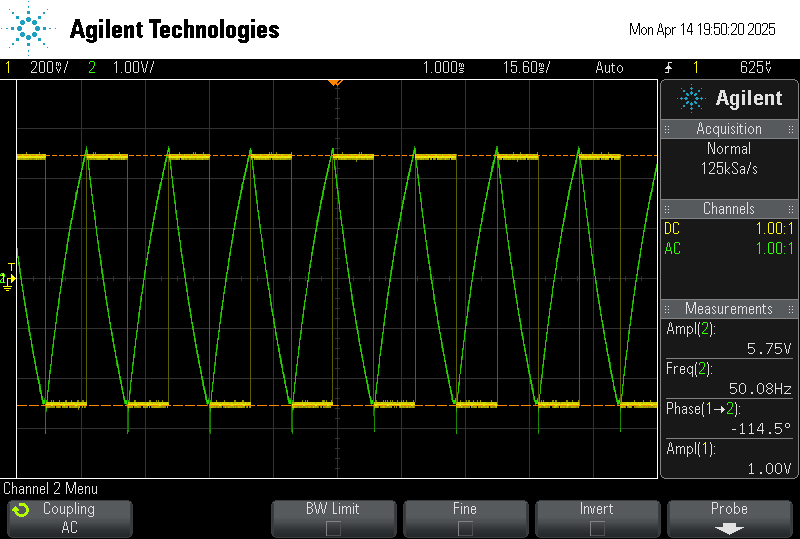
\includegraphics[width =0.85\textwidth]{figures/integrator_rechteck.png}
    \caption{Rechtecksignal und Integratorausgangssignal.}
    \label{fig:integrator_rechteck}
\end{figure}

\begin{figure}[h!]
    \centering
    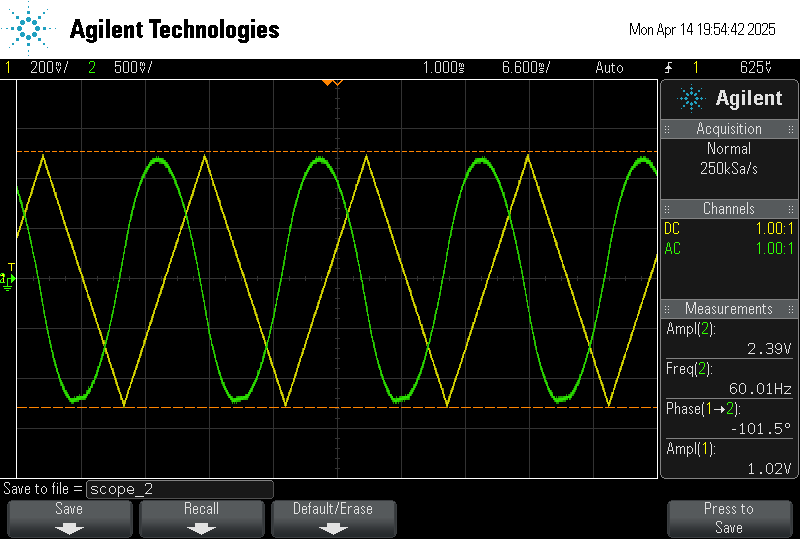
\includegraphics[width =0.85\textwidth]{figures/integrator_dreieck.png}
    \caption{Dreiecksignal und Integratorausgangssignal.}
    \label{fig:integrator_dreieck}
\end{figure}

\newpage

\subsection{Differenzierer}
\label{sec:Differenzierer_Auswertung}

Der Differenzierer wurde gemäß \autoref{fig:differenzierer} aufgebaut.
Es wurde der Widerstand $R = \qty{100}{\kilo\ohm}$ und die Kapazität $C = \qty{22}{\nano\farad}$ verwendet, was eine Zeitkonstante \newline
$\tau = RC = \qty{2.20e-3}{\second}$ liefert.


Auch hier wurde das Bode-Diagramm aufgenommen. Der gemessene Verlauf zeigt das erwartete lineare Ansteigen der Verstärkung mit der Frequenz, 
wie es für einen idealen Differentiator charakteristisch ist.

Der Verlauf in \autoref{plt:differenzierer} zeigt das erwartete 
lineare ansteigen proportional zu $f$ eines idealen Differenzierers,
dabei ist $A_{0,\text{theorie}} = 2 \pi R C$.

\begin{figure}[h!]
    \centering
    \includegraphics[width=\textwidth]{differentiator.pdf}
    \caption{Bode-Diagramm des Differenzierers mit $A_0 * f$ in $\unit{dB}$ auf der y-Achse und $f$ auf der x-Achse.}
    \label{plt:differenzierer}
\end{figure}

Gemäß \autoref{eq:differenzierer} ist das Ausgangssignal eines Differenzierers proportional zur
Ableitung des Eingangssignals. In \autoref{fig:differenzierer_rechteck} und
\autoref{fig:differenzierer_dreieck} ist die Signalspannung jeweils in Gelb und das Ausgangssignal in
Grün dargestellt.
\newpage

\begin{figure}[h!]
    \centering
    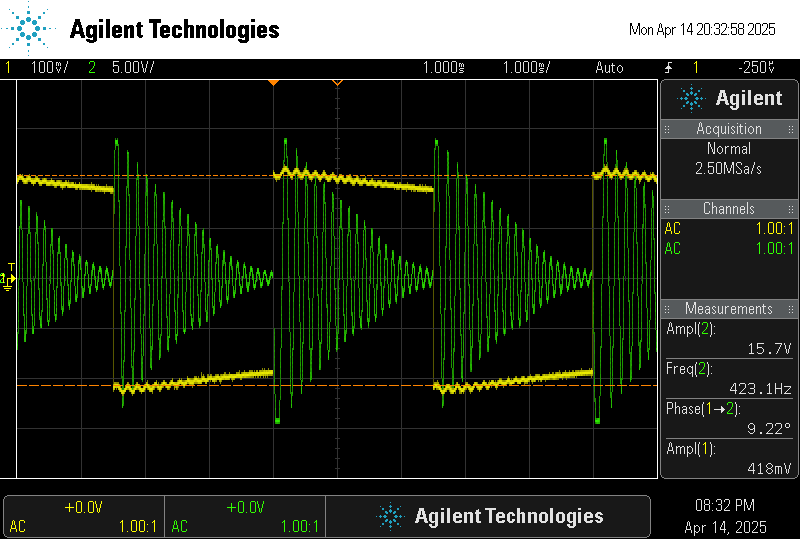
\includegraphics[width =0.85\textwidth]{figures/differenzierer_rechteck.png}
    \caption{Rechtecksignal und Differenziererausgangssignal.}
    \label{fig:differenzierer_rechteck}
\end{figure}

\begin{figure}[h!]
    \centering
    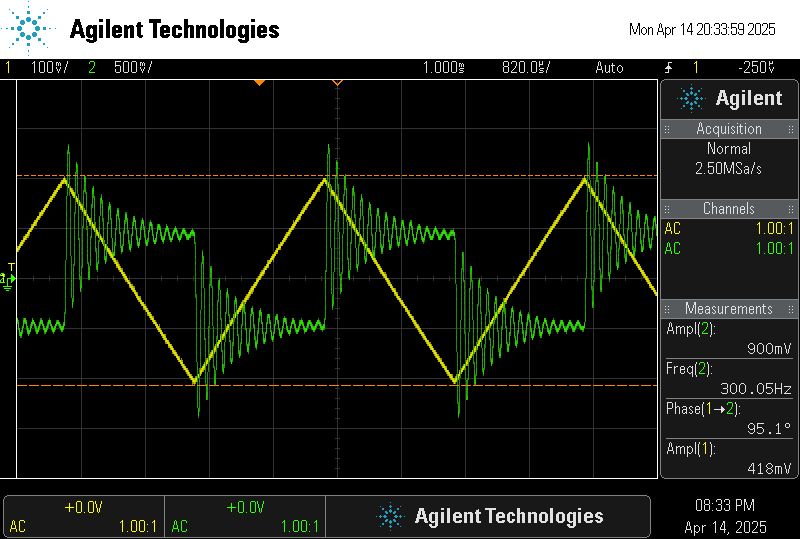
\includegraphics[width =0.85\textwidth]{figures/differenzierer_dreieck.png}
    \caption{Dreiecksignal und Differenziererausgangssignal.}
    \label{fig:differenzierer_dreieck}
\end{figure}

% Integrator messdaten
\begin{table}
    \centering
    \caption{Messdaten zum Integrator.}
    \label{tab:integrator}
    \resizebox{0.8\textwidth}{!}{%
    \begin{tblr}{
        colspec = {
            S[table-format=2.2]
            S[table-format=3.2]
            S[table-format=2.2]
            S[table-format=3.2]
            S[table-format=2.2]
            S[table-format=3.2]
        },
        row{1} = {guard},
        row{2} = {guard, mode = math}
    }
        \toprule
        \SetCell[c=2]{c} \textbf{Messpunkte 1-9} && \SetCell[c=2]{c} \textbf{Messpunkte 10-19} && \SetCell[c=2]{c} \textbf{Messpunkte 19-25} & \\
        \cmidrule[lr]{1-2} \cmidrule[lr]{3-4} \cmidrule[lr]{5-6}
        U_\text{out} \mathbin{/} \unit{\volt} & f \mathbin{/} \unit{\hertz} & 
        U_\text{out} \mathbin{/} \unit{\volt} & f \mathbin{/} \unit{\hertz} & 
        U_\text{out} \mathbin{/} \unit{\volt} & f \mathbin{/} \unit{\hertz} \\
        \midrule
            11.5 & 5  & 3.66 & 50  & 0.48          & 500           \\
            10.5 & 10 & 3.14 & 60  & 0.43          & 600           \\
            8.8  & 15 & 2.69 & 70  & 0.39          & 700           \\
            7.6  & 20 & 2.41 & 80  & 0.35          & 800           \\
            6.8  & 25 & 2.17 & 90  & 0.33          & 900           \\
            5.8  & 30 & 2.01 & 100 & 0.31          & 1000          \\
            5.2  & 35 & 1.04 & 200 & 0.31          & 2000          \\
            4.8  & 40 & 0.74 & 300 & $\mathbin{/}$ & $\mathbin{/}$ \\
            3.98 & 45 & 0.58 & 400 & $\mathbin{/}$ & $\mathbin{/}$ \\
        \bottomrule        	
    \end{tblr}
    }
\end{table}

% Differenzierer Messdaten
\begin{table}
    \centering
    \caption{Messdaten zum Differenzierer.}
    \label{tab:Differenzierer}
    \resizebox{0.8\textwidth}{!}{%
    \begin{tblr}{
        colspec = {
            S[table-format=2.2]
            S[table-format=3.2]
            S[table-format=2.2]
            S[table-format=3.2]
            S[table-format=2.2]
            S[table-format=3.2]
        },
        row{1} = {guard},
        row{2} = {guard, mode = math}
    }
        \toprule
        \SetCell[c=2]{c} \textbf{Messpunkte 1-5} && \SetCell[c=2]{c} \textbf{Messpunkte 6-10} && \SetCell[c=2]{c} \textbf{Messpunkte 11-15} & \\
        \cmidrule[lr]{1-2} \cmidrule[lr]{3-4} \cmidrule[lr]{5-6}
        U_\text{out} \mathbin{/} \unit{\volt} & f \mathbin{/} \unit{\kilo\hertz} & 
        U_\text{out} \mathbin{/} \unit{\volt} & f \mathbin{/} \unit{\kilo\hertz} & 
        U_\text{out} \mathbin{/} \unit{\volt} & f \mathbin{/} \unit{\kilo\hertz} \\
        \midrule
            0.065 & 0.03 & 0.370 & 0.30 & 0.960 & 0.80 \\
            0.087 & 0.05 & 0.490 & 0.40 & 1.090 & 0.90 \\
            0.115 & 0.07 & 0.600 & 0.50 & 1.190 & 1.00 \\
            0.145 & 0.10 & 0.740 & 0.60 & 2.390 & 2.00 \\
            0.257 & 0.20 & 0.840 & 0.70 & 3.680 & 3.00 \\
        \bottomrule        	
    \end{tblr}
    }
\end{table}

\subsection{Schmitt Trigger}
Aus \autoref{eq:SchmittTriggerSchaltschwelle} und den Komponenteneigenschaften aus \autoref{subsec:SchmittTrigger} 
kann der theoretische Wert berechnet $T_\text{theo} = \qty{29.89}{\volt}$ und mit dem experimentellen Wert $T_\text{exp}~=~\qty{28.1}{\volt}$
verglichen werden, woraus eine Abweichung von $\qty{6.00}{\percent}$ folgt. 

\subsection{Generator}
Der Theoretische Wert der Frequenz, welcher aus \autoref{eq:GeneratorFrequenz} berechnet wird, beträgt $f_\text{theo} = \qty{2.5}{\kilo\hertz}$.
Der Experimentelle Wert von $f_\text{exp} = \qty{1.67}{\kilo\hertz}$ weicht um $\qty{33.2}{\percent}$ vom Theorie Wert ab.

\subsection{Generator mit variierender Amplitude}
\label{sec:Generator_Auswertung}
Der Generator mit variierender Amplitude wurde gemäß \autoref{fig:generator} 
aufgebaut. Dabei wurden die Widerstände $R = \qty{10}{\kilo\ohm}$ und $R_1 = \qty{10}{\kilo\ohm}$ und für den Kondensatoren 
eine Kapazität $C = \qty{100}{\nano\farad}$.
Mittels eines Rechtecksignals wurden die Schwingungen des Generators angeregt. In \autoref{fig:generator_1} ist die Messung
der Schwingungen dargestellt. Dabei ist die Rechteckspannung in Gelb und die Ausgangsspannung in Grün dargestellt.

\begin{figure}
    \centering
    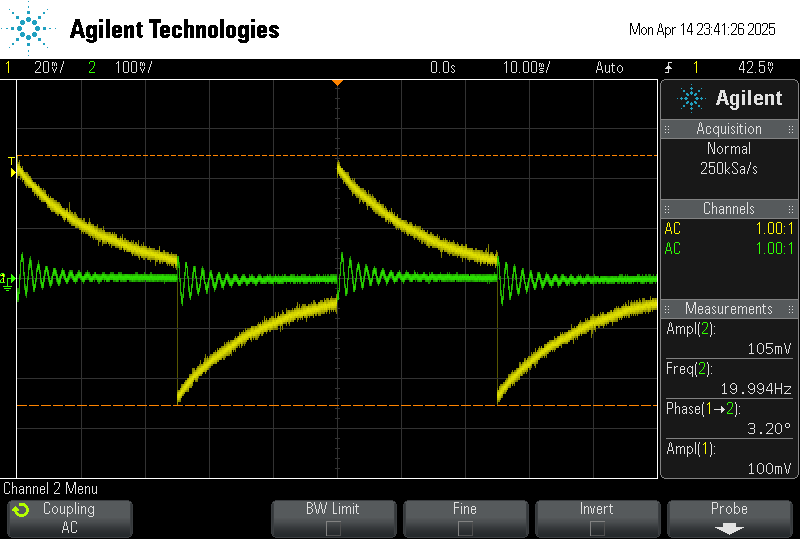
\includegraphics[width =\textwidth]{figures/scope_10.png}
    \caption{Angeregte Schwingungen am Generator mit variierender Amplitude.}
    \label{fig:generator_1}
\end{figure}

Gemäß \autoref{eq:GeneratorMitVariierenderAmplitudeLoesung} erwartet man einen exponentiellen
Abfall der Amplitude mit der Zeit. Dies kann durch den Zusammenhang

\begin{equation*}
    A(t) = A_0 \, \exp(-\frac{t}{\tau})
\end{equation*}

modelliert werden. Durch das logarithmieren dieser Gleichung ergibt sich die Geradengleichung

\begin{equation*}
    \ln(A(t)) = \ln(A_0) - \frac{t}{\tau}.
\end{equation*}

Es wird nun eine lineare Regression auf die logarithmierten Werte der Amplitude durchgeführt.
Die Amplitudenwerte werden für eine Anregung in \autoref{fig:generator_1}
abgelesen und in \autoref{tab:generator_1} aufgelistet.

\begin{table}
    \centering
    \caption{Zeitlicher Verlauf der Amplitude am Generator mit variierender Amplitude.}
    \label{tab:generator_1}
    \sisetup{table-format = 2.2} 
    \begin{tblr}{
        colspec = {S S S S S S},
        row{1} = {guard, mode = math}
    }
        \toprule 
        t \mathbin{/} \unit{\milli\second} & A \mathbin{/} \unit{\milli\volt} & \ln(U) &
        t \mathbin{/} \unit{\milli\second} & A \mathbin{/} \unit{\milli\volt} & \ln(U)  \\
        \midrule
        0.10  & 51.04 & -2.98 & 12.85 & 34.26 & -3.37 \\
        0.70  & 58.10 & -2.85 & 13.50 & 34.03 & -3.38 \\
        1.45  & 47.42 & -3.05 & 14.10 & 34.96 & -3.35 \\
        1.95  & 52.02 & -2.96 & 14.75 & 30.01 & -3.51 \\
        2.70  & 47.78 & -3.04 & 15.35 & 33.81 & -3.39 \\
        3.25  & 52.58 & -2.95 & 15.95 & 29.66 & -3.52 \\
        3.85  & 46.32 & -3.07 & 16.60 & 32.60 & -3.42 \\
        4.50  & 50.97 & -2.98 & 17.30 & 30.72 & -3.48 \\
        5.20  & 46.17 & -3.08 & 17.90 & 29.48 & -3.52 \\
        5.85  & 46.14 & -3.08 & 18.50 & 26.75 & -3.62 \\
        6.50  & 43.76 & -3.13 & 19.20 & 32.50 & -3.43 \\
        7.05  & 43.18 & -3.14 & 19.80 & 25.24 & -3.68 \\
        7.80  & 37.53 & -3.28 & 20.45 & 30.19 & -3.50 \\
        8.30  & 42.88 & -3.15 & 21.10 & 25.94 & -3.65 \\
        9.00  & 41.44 & -3.18 & 21.75 & 29.43 & -3.53 \\
        9.60  & 38.15 & -3.27 & 22.40 & 23.63 & -3.75 \\
        10.30 & 36.67 & -3.31 & 22.95 & 24.21 & -3.72 \\
        10.85 & 36.39 & -3.31 & 23.70 & 21.92 & -3.82 \\
        11.55 & 35.92 & -3.33 & 24.20 & 26.12 & -3.65 \\
        12.20 & 38.05 & -3.27 & 24.90 & 20.41 & -3.89 \\
        \bottomrule
    \end{tblr}
\end{table}

Die lineare Regression auf die logarithmierten Werte ist in \autoref{plt:generator_1_regression} 
dargestellt und ergibt die Parameter

\begin{equation}
    \tau_{\text{exp}} = \qty{288(12)}{\milli\second} \quad \text{und} \quad \ln(A_0) = \num{-2.91(0.02)}.
\end{equation}

\begin{figure}
    \centering
    \includegraphics[width =\textwidth]{build/generator_tau.pdf}
    \caption{Lineare Regression auf die logarithmierten Werte der Amplitude am Generator mit variierender Amplitude.}
    \label{plt:generator_1_regression}
\end{figure}

Der theoretische Wert $\tau_{\text{theo}}$ wird mit \autoref{eq:generatorMitVariierenderAmplitude} 
unter der Annahme $\abs{\eta} = 1$ berechnet und beträgt

\begin{equation}
    \tau_{\text{theo}} = \qty{200}{\milli\second}.
\end{equation}
\section{Diskussion}
\label{sec:Diskussion}

In diesem Abschnitt werden die Ergebnisse der Versuche diskutiert und mögliche Fehlerquellen
aufgezeigt.

\subsection{Invertierender Verstärker}
In der \ref{subsec:Auswertung_InvertierenderVerstaerker} wurden Abweichungen von unter $\qty{3.5}{\percent}$ gemessen. 
Außerdem weisen die \autoref{plt:invertierenderVerstaerker1}, \ref{plt:invertierenderVerstaerker2} und \ref{plt:invertierenderVerstaerker3}  einen 
zu erwartenden Verlauf auf und lassen sich gut an eine typische Low Pass Filter Funktion \ref{eq:lowPassFilter} fitten.
Die Messungen bestätigen somit die Theoretischen Erwartungen.

\subsection{Integrator}
\label{sec:Integrator_Diskussion}
Die \autoref{plt:integrator} zeigt, dass die Messdaten nicht exakt einem linearen Verlauf folgen. 
Aufgrund der niedrigen Frequenzen kann dies vermutlich auf Untergrundeffekte und allgemeine Schwierigkeiten bei der Darstellung eines sauberen Signals auf dem Oszilloskop zurückgeführt werden.
Zudem könnten Messunsicherheiten in den Bauteilen zu größeren Abweichungen führen.
Im Bereich von etwa $\qty{20}{\hertz}$ bis $\qty{60}{\hertz}$ zeigt sich jedoch ein Verhalten, das dem theoretischen Verlauf besser entspricht.
Dieser Frequenzbereich ist allerdings zu schmal, um eine aussagekräftige Analyse ausschließlich auf ihn zu stützen.
Die experimentell bestimmte Verstärkung weicht um $\qty{25.41}{\percent}$ vom theoretisch erwarteten Wert ab, was innerhalb der Toleranzen der Bauteileigenschaften und der allgemeinen Messunsicherheiten liegt.

Anhand von \autoref{fig:integrator_rechteck} und 
\autoref{fig:integrator_dreieck} ist qualitativ zu 
erkennen, dass das Ausgangssignal des Integrators, bis auf einen Vorfaktor, dem zeitlichen Integral 
des Eingangssignals entspricht. Aus dem Rechtecksignal ergibt sich ein Dreieckssignal und aus dem
Dreieckssignal ein Parabelsignal. Dies entspricht den Erwartungen gemäß \autoref{eq:integrator}.

\subsection{Differenzierer}
\label{sec:Differenzierer_Diskussion}
Die \autoref{plt:differenzierer} zeigt einen linearen Verlauf für höhere Frequenzen und verliert im unteren Frequenzbereich leicht an Linearität.
Dies lässt sich auf Untergrundeffekte zurückführen, da im niedrigen Frequenzbereich die Verstärkung abnimmt und dadurch Hintergrundstörungen dominanter werden.
Dies führt dazu, dass die Fit-Funktion auf natürliche Weise leicht nach oben verschoben wird.
Zukünftige Analysen könnten daher versuchen, den Untergrund im Vorfeld zu messen und rechnerisch zu subtrahieren.
Eine Abweichung von $\qty{7.51}{\percent}$ vom theoretischen Wert bestätigt insgesamt die theoretische Erwartung.

In \autoref{fig:differenzierer_rechteck} und
\autoref{fig:differenzierer_dreieck} sind die Eingangs-
und Ausgangssignale des Differenzierers dargestellt. Es wird erwartet, dass an den Sprüngen des
Rechtecksignals die Amplitude des Differenzierersignals einen Peak zeigt. Dies ist 
in \autoref{fig:differenzierer_rechteck} zu erkennen.
Es sei angemerkt, dass die Spannungsausschläge gedämpfte Schwingungen im Schaltkreis anregen, sodas
die Peaks nicht ideal sind und zu den beobachteten Schwingungen führen.
Ein ähnliches Verhalten ist auch im Fall des Dreiecksignals zu beobachten. Hierbei springt 
das Ausgangssignal zwischen zwei Werten hin und her, wobei ebenfalls gedämpfte Schwingungen
angeregt werden. Bis auf die gedämpften Schwingungen entspricht das Ausgangssignal des Differenzierers
somit den Erwartungen gemäß \autoref{eq:differenzierer}.

\subsection{Generator}
Die gemessene Frequenz von $f_\text{exp} = \qty{1.67}{\kilo\hertz}$ weicht um $\qty{33.2}{\percent}$ vom theoretischen Wert $f_\text{theo} = \qty{2.5}{\kilo\hertz}$ ab.  
Diese Differenz kann durch Bauteiltoleranzen, insbesondere beim Kondensator, sowie durch nicht-ideale Eigenschaften der Operationsverstärker und Versorgungsspannungen erklärt werden.  
Trotz der Abweichung liegt der Wert in einer realistischen Größenordnung und bestätigt qualitativ das erwartete Oszillationsverhalten.

\subsection{Generator mit variierender Amplitude}
\label{sec:Generator_Diskussion}
Der experimentelle Wert und die theoretische Vorhersage für $\tau$ passen im Rahmen der Unsicherheiten nicht zusammen.
Dies kann jedoch dadurch erklärt werden, dass der Wert von $\abs{\eta}$ durch das Potentiometer eingestellt wird und nicht bekannt 
ist. Der theoretische Wert liegt unterhalb des experimentellen Wertes. Dies deutet darauf hin, 
dass gemäß \autoref{eq:generatorMitVariierenderAmplitude} der Wert von $\abs{\eta}$ kleiner ist als der 
angenommene Wert von $\abs{\eta} = 1$.

\printbibliography{}
\section*{Anhang}
\addcontentsline{toc}{section}{Anhang}
\begin{figure}[H]
  \centering
  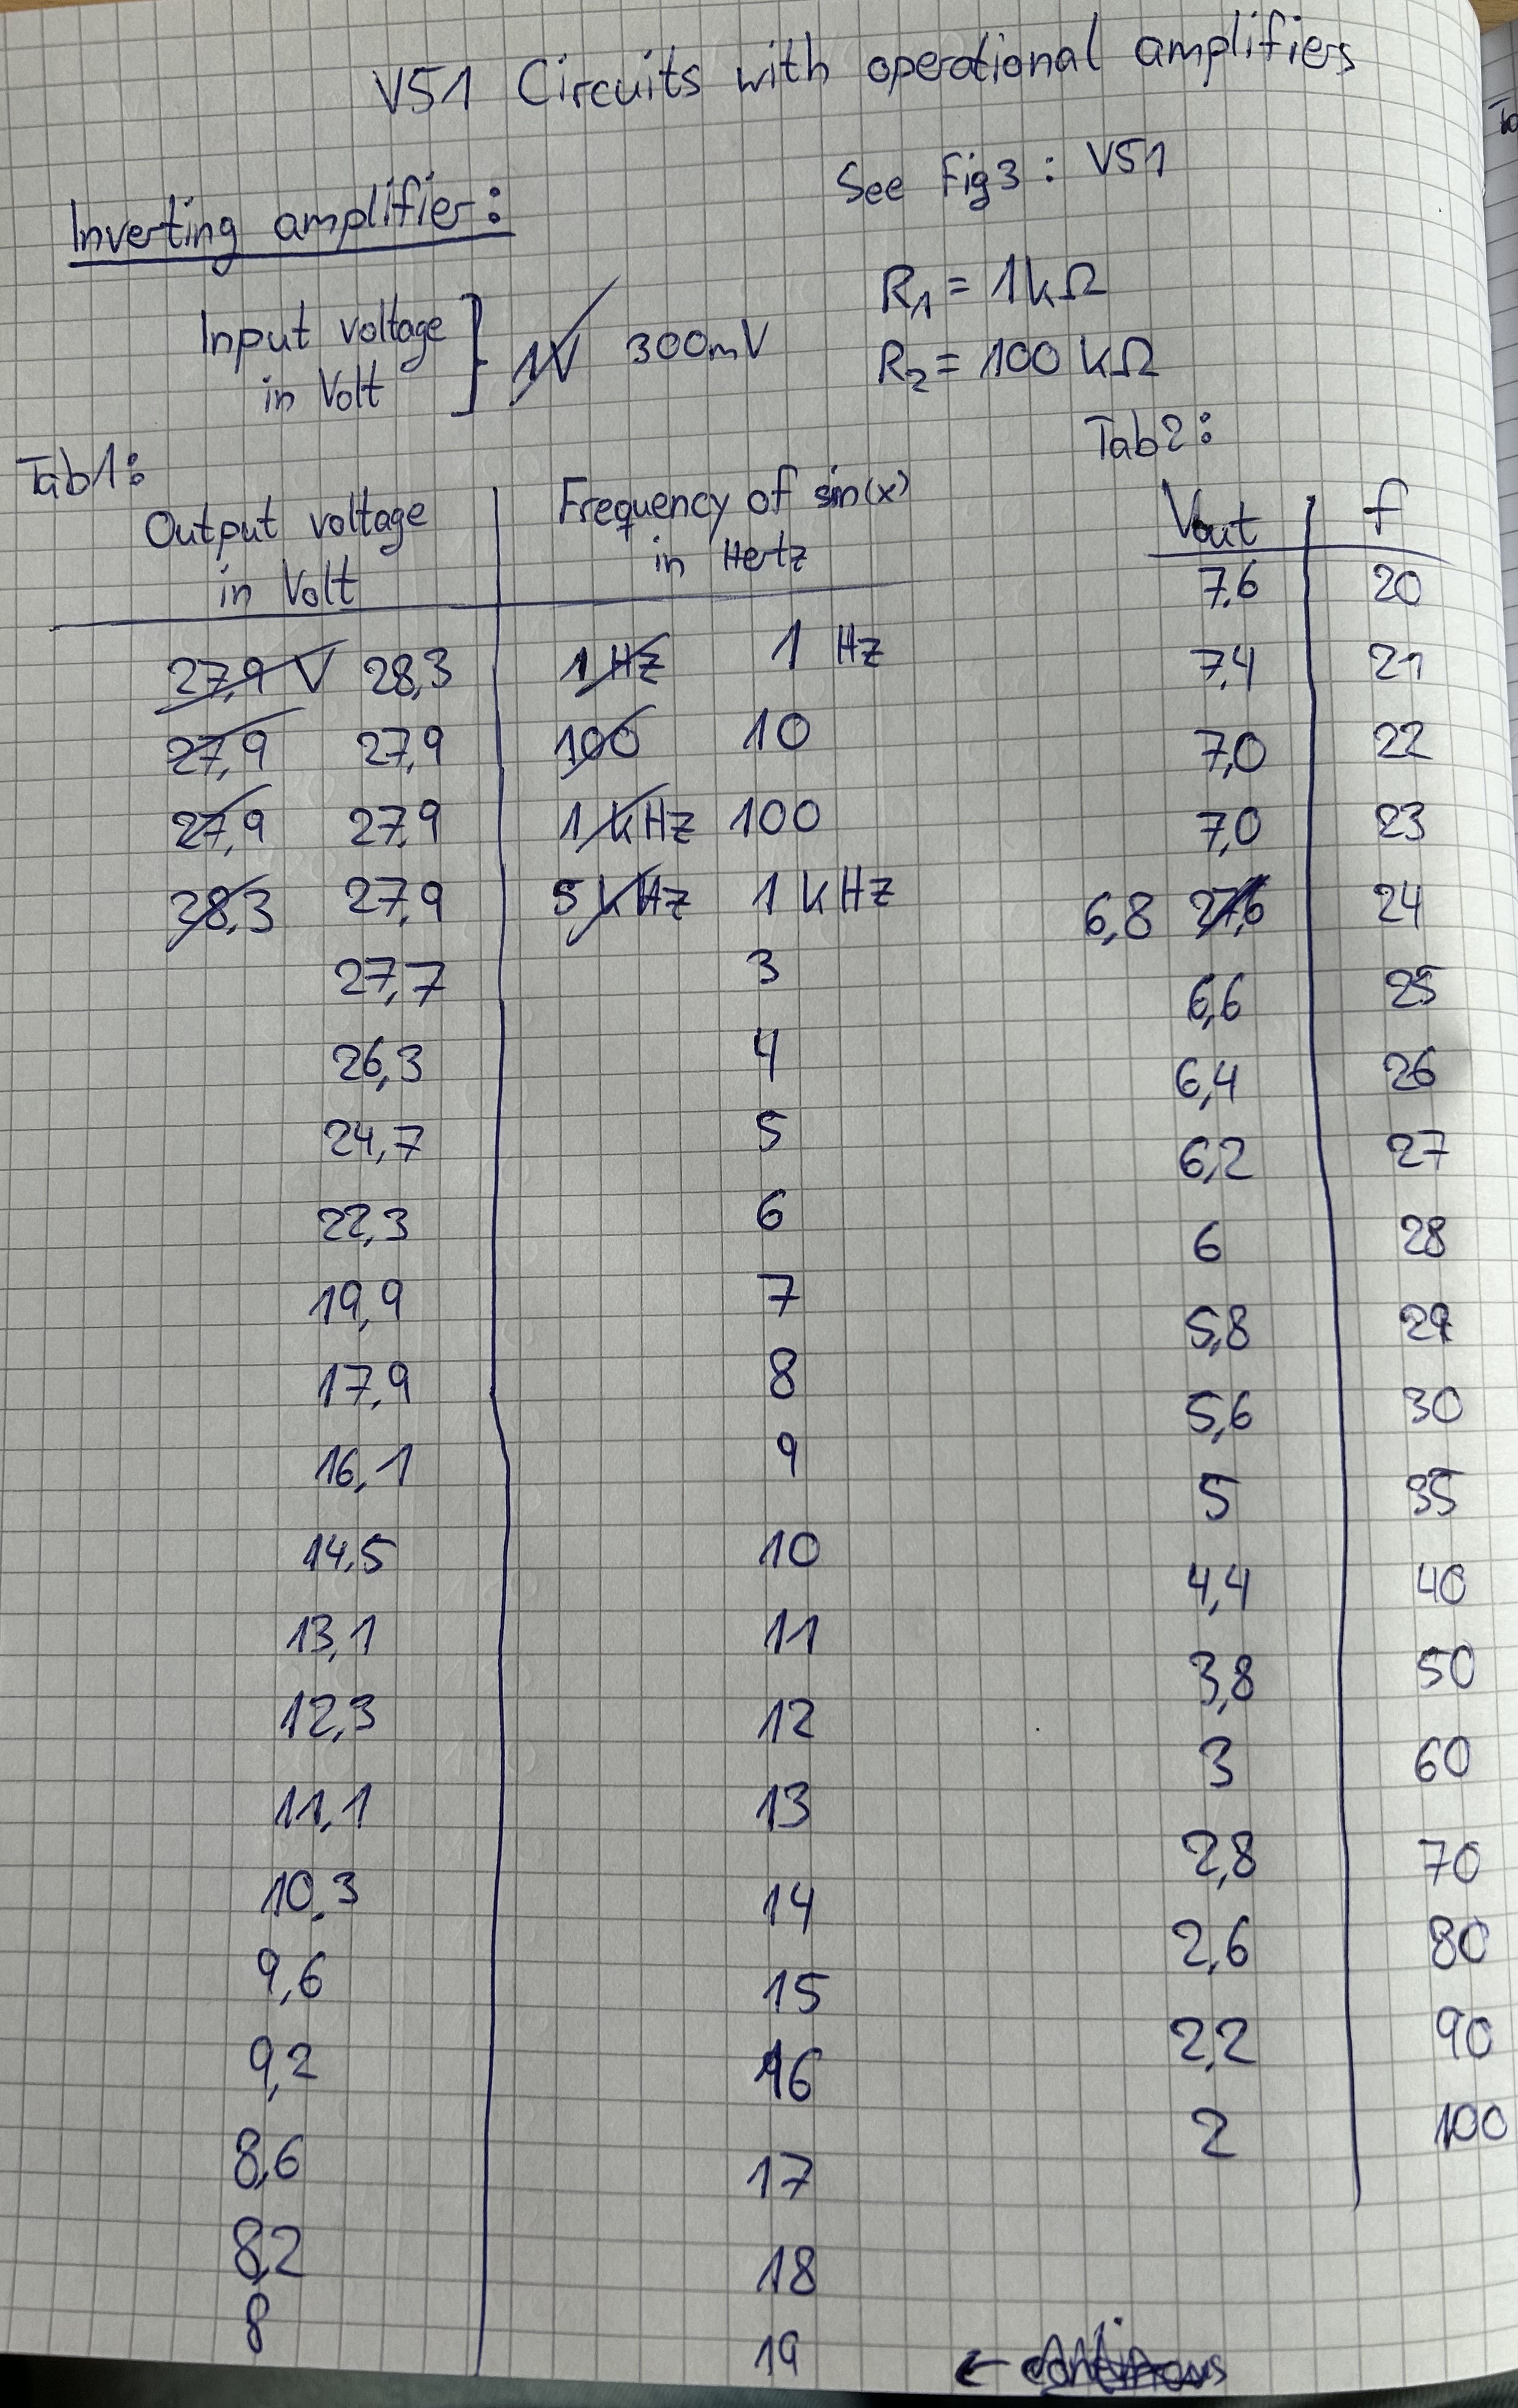
\includegraphics[width = 0.75\textwidth]{figures/Messdaten1.jpeg}
\end{figure}
\begin{figure}
  \centering
  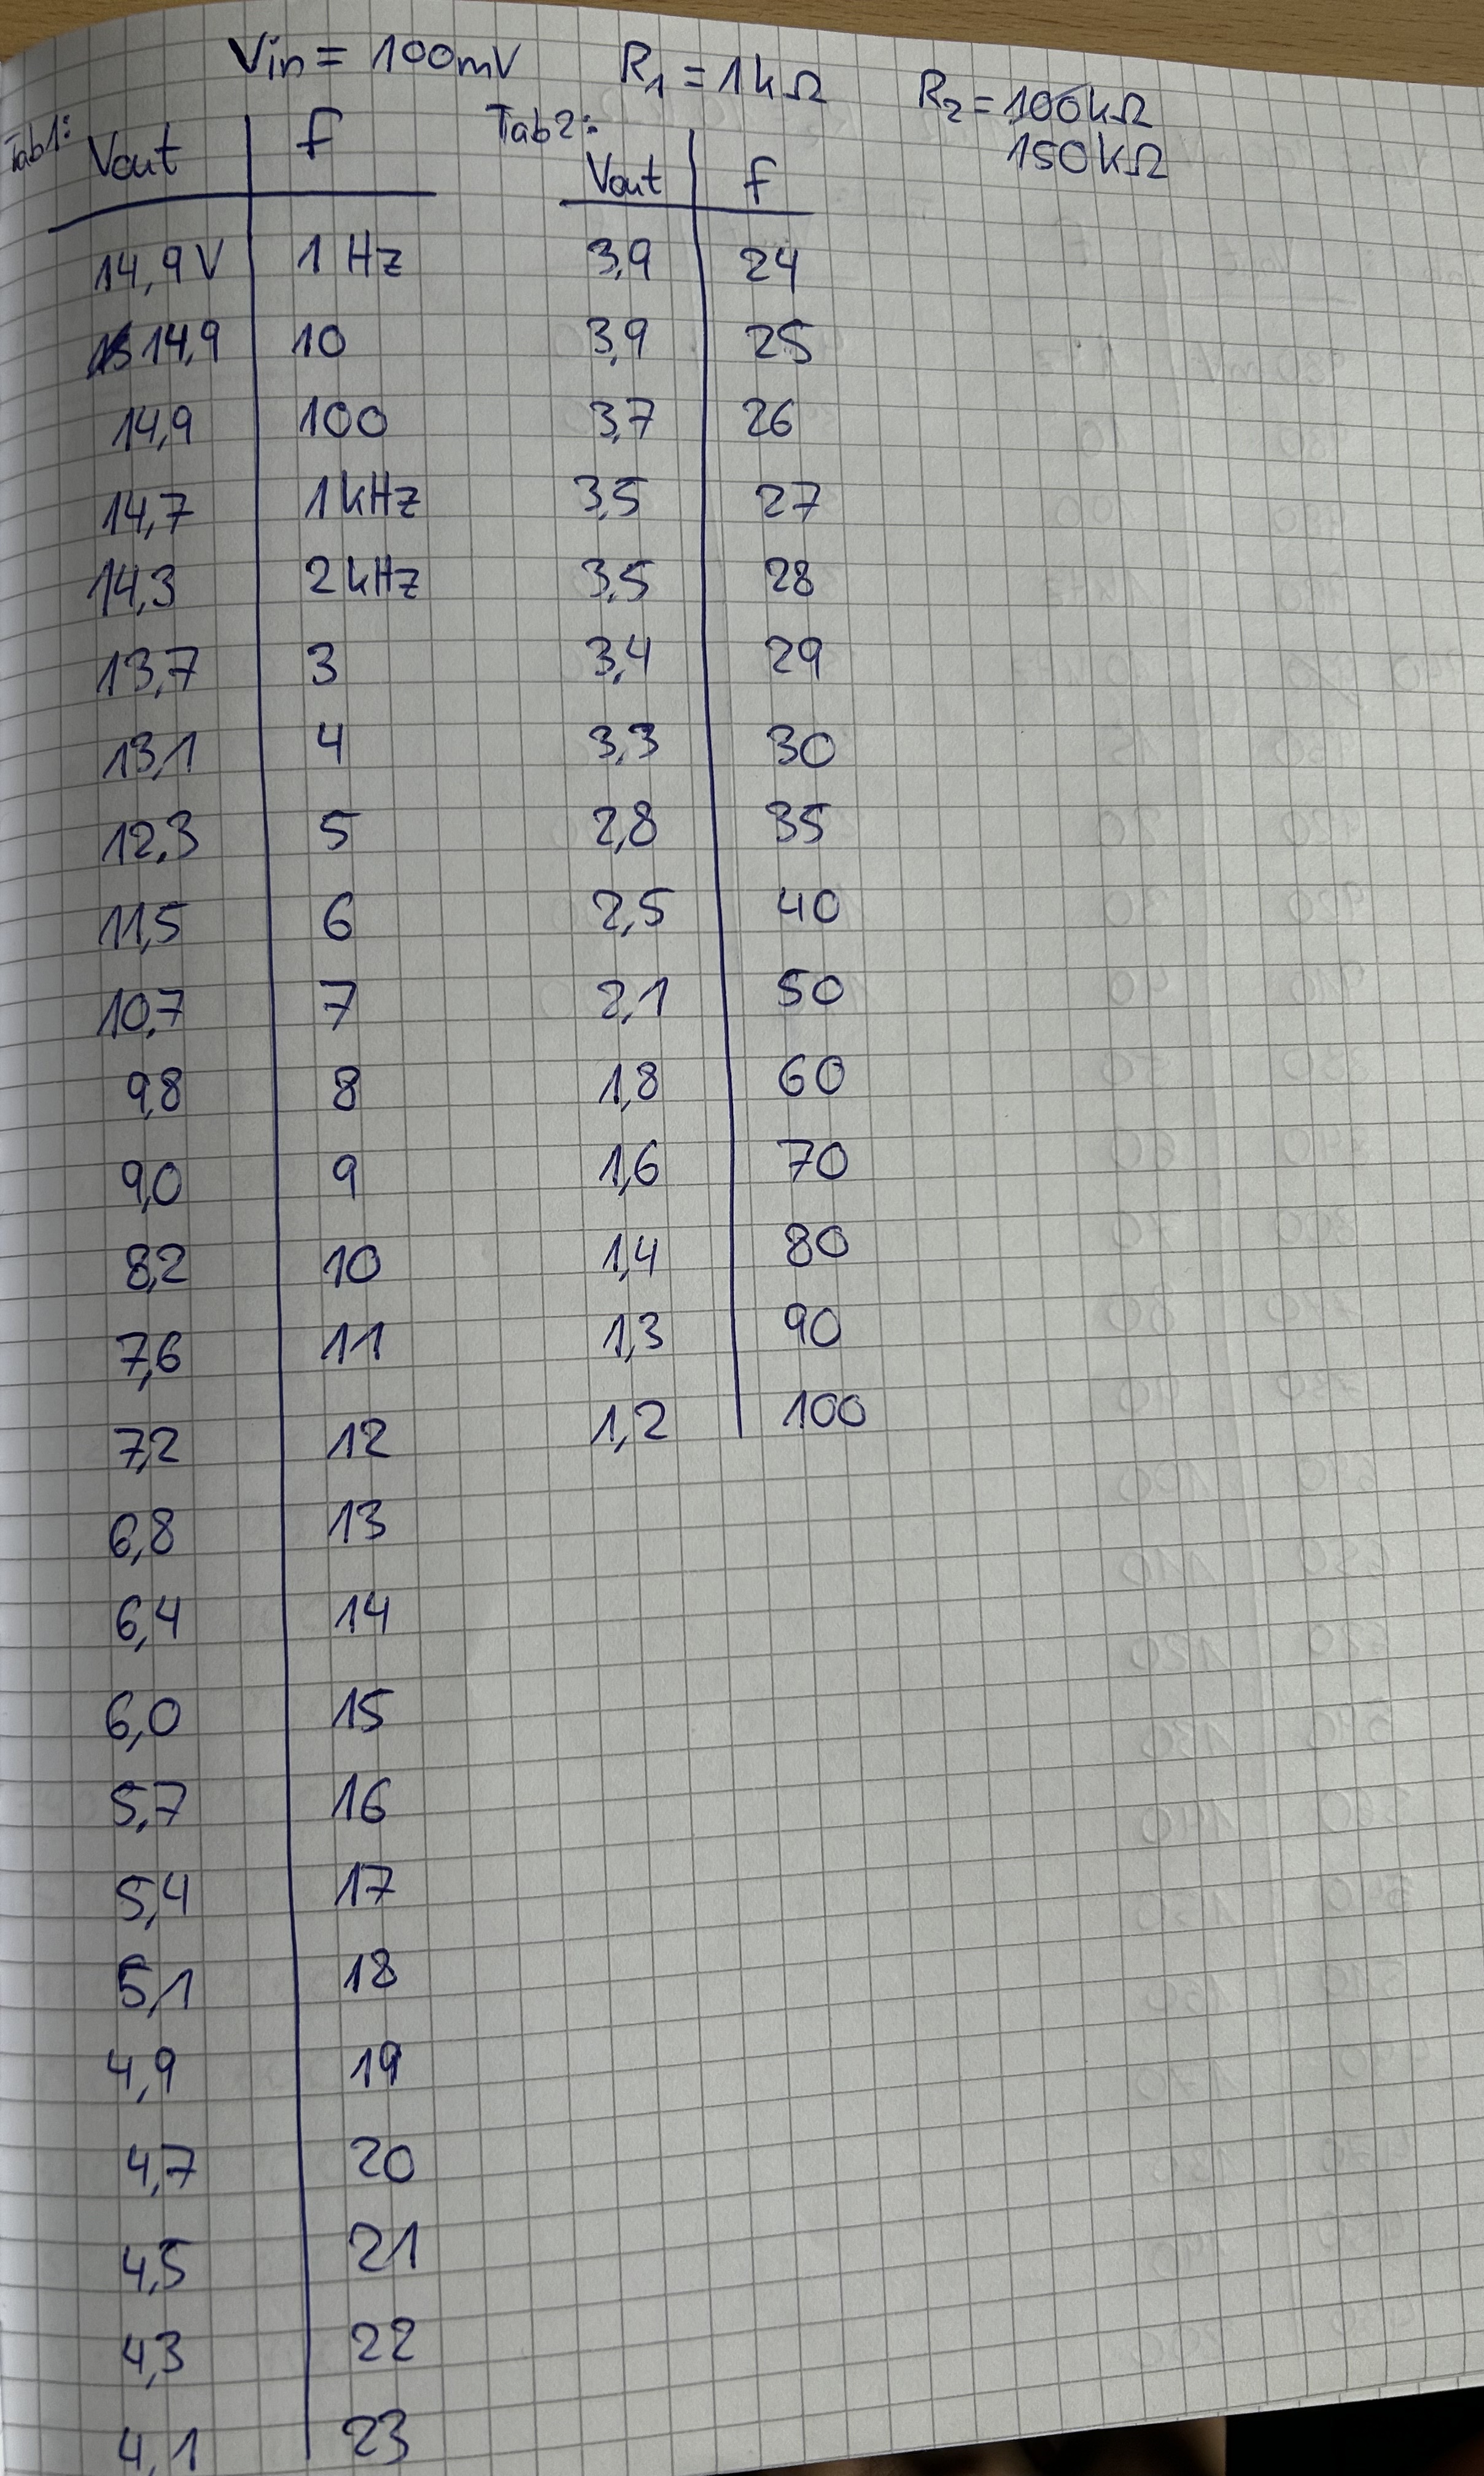
\includegraphics[width = 0.9\textwidth]{figures/Messdaten2.jpeg}
\end{figure}
\begin{figure}
  \centering
  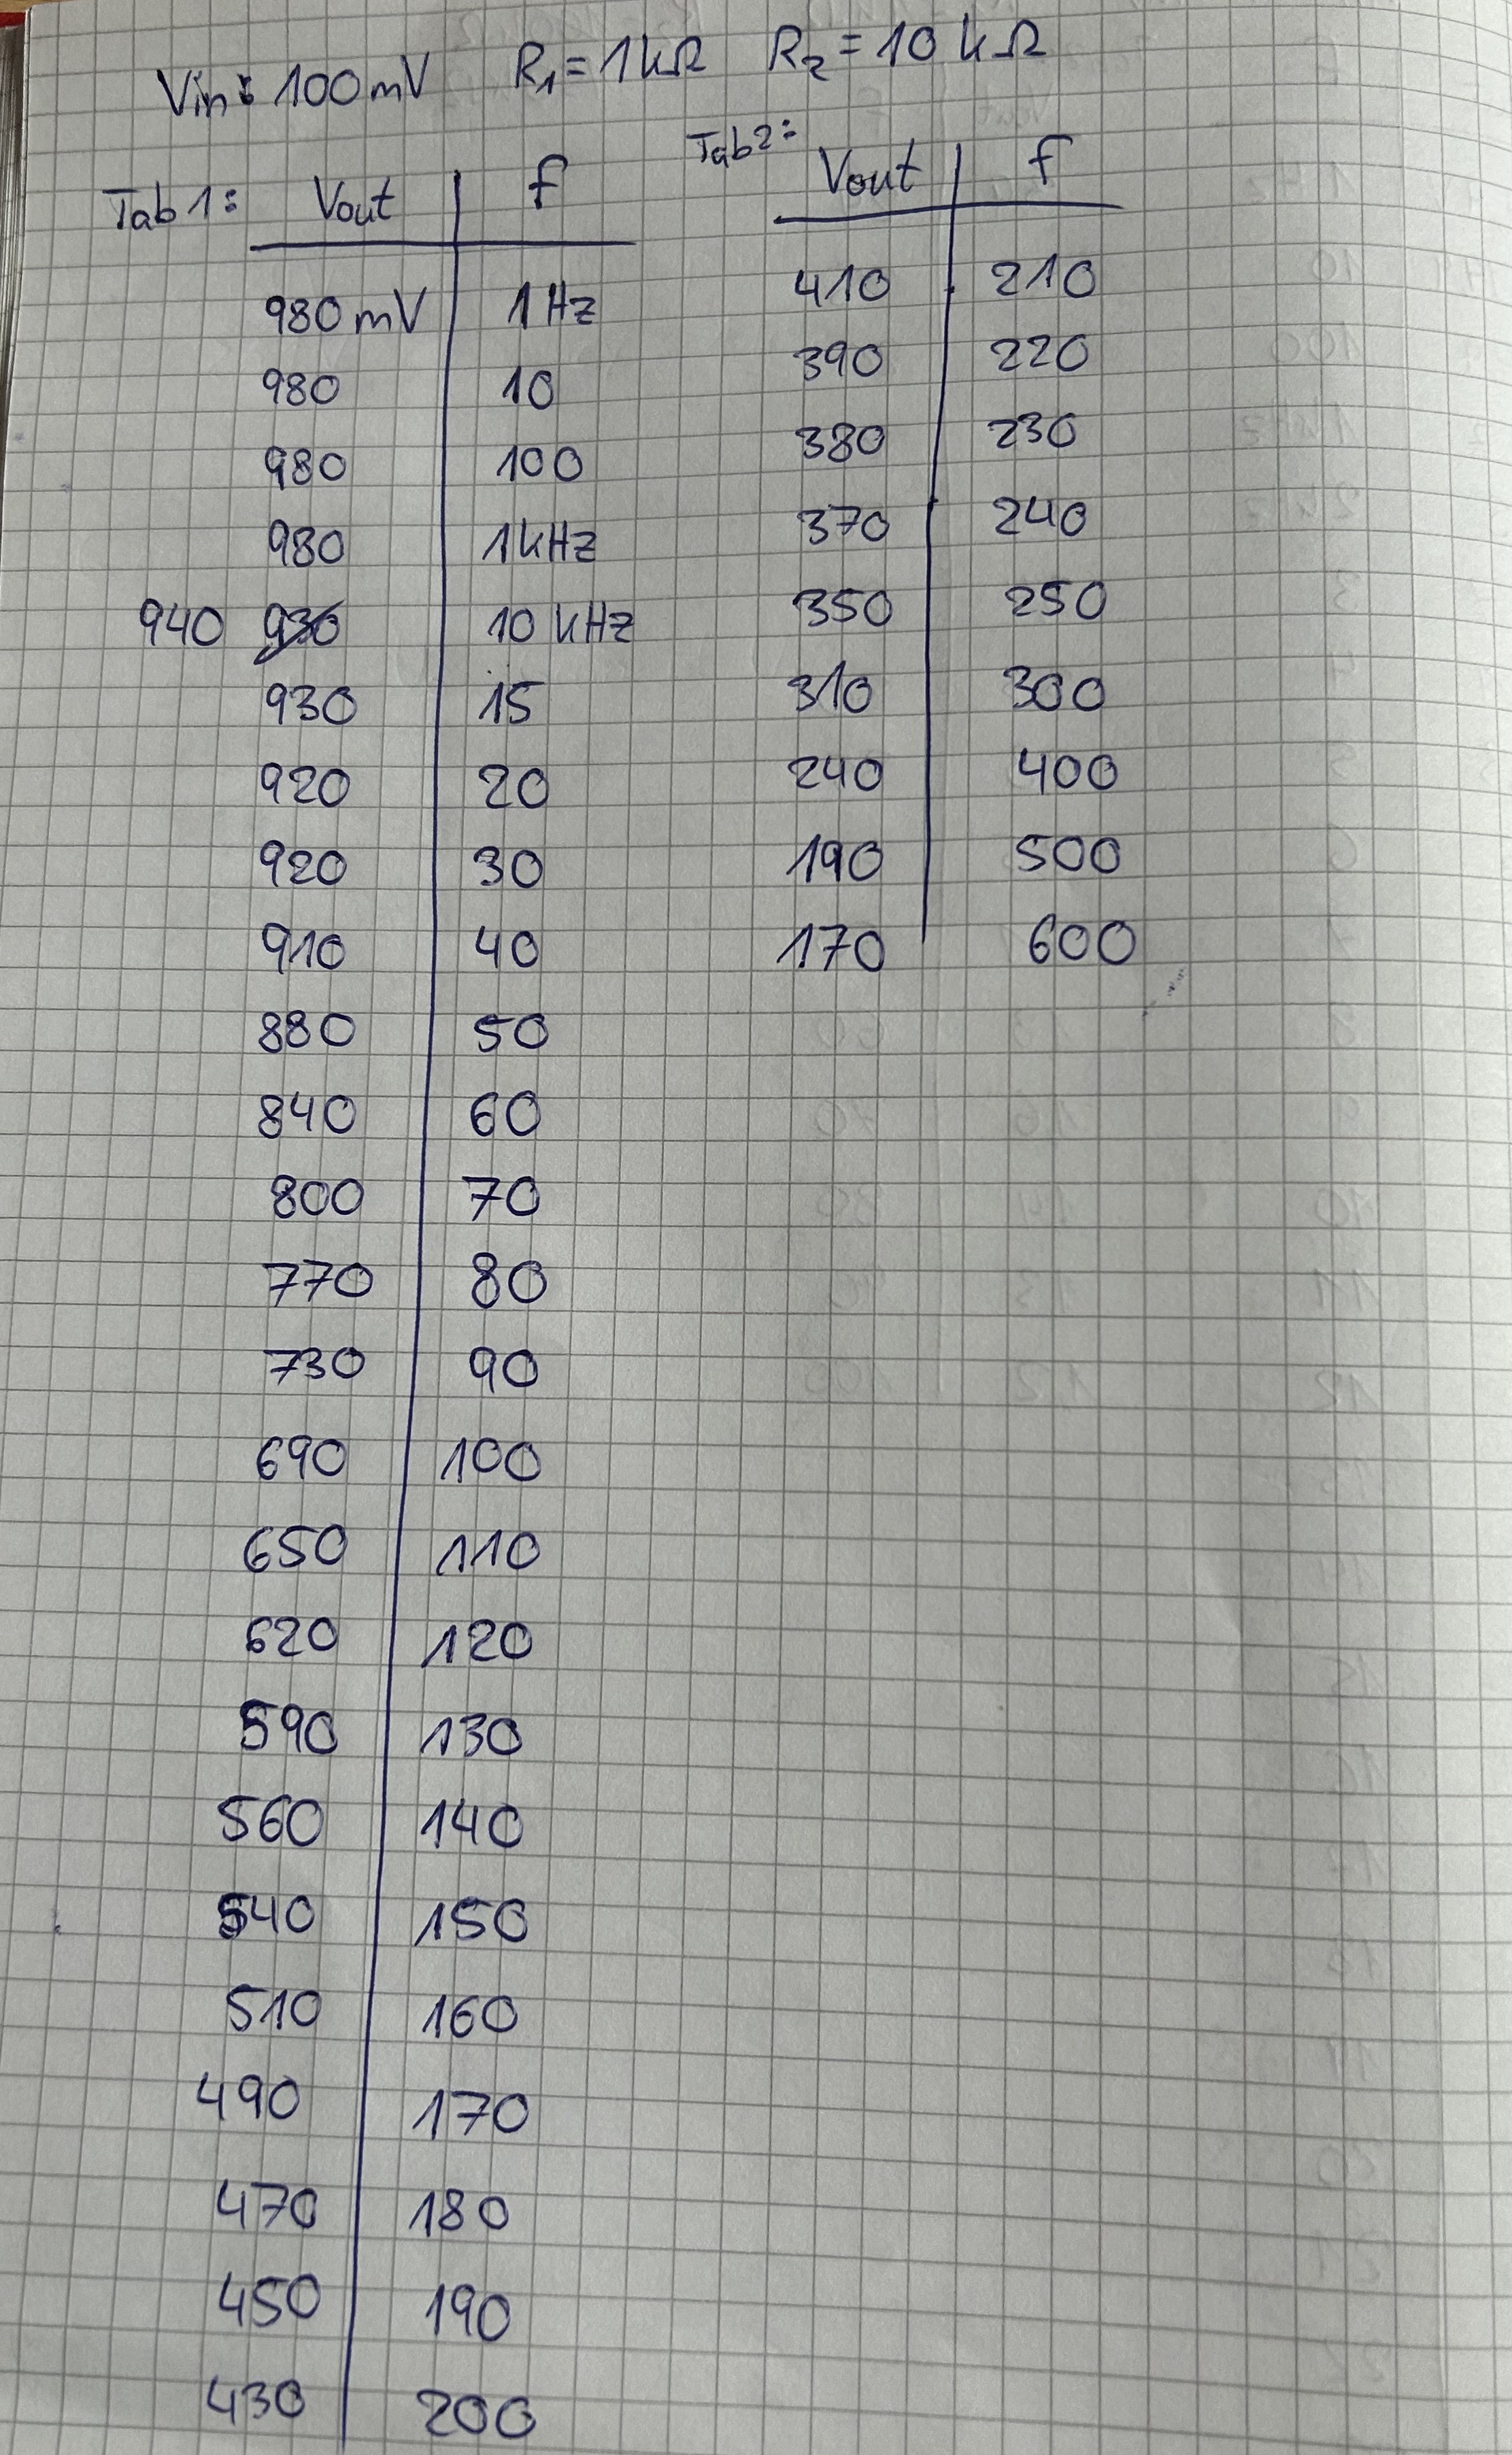
\includegraphics[width = 0.9\textwidth]{figures/Messdaten3.jpeg}
\end{figure}
\begin{figure}
  \centering
  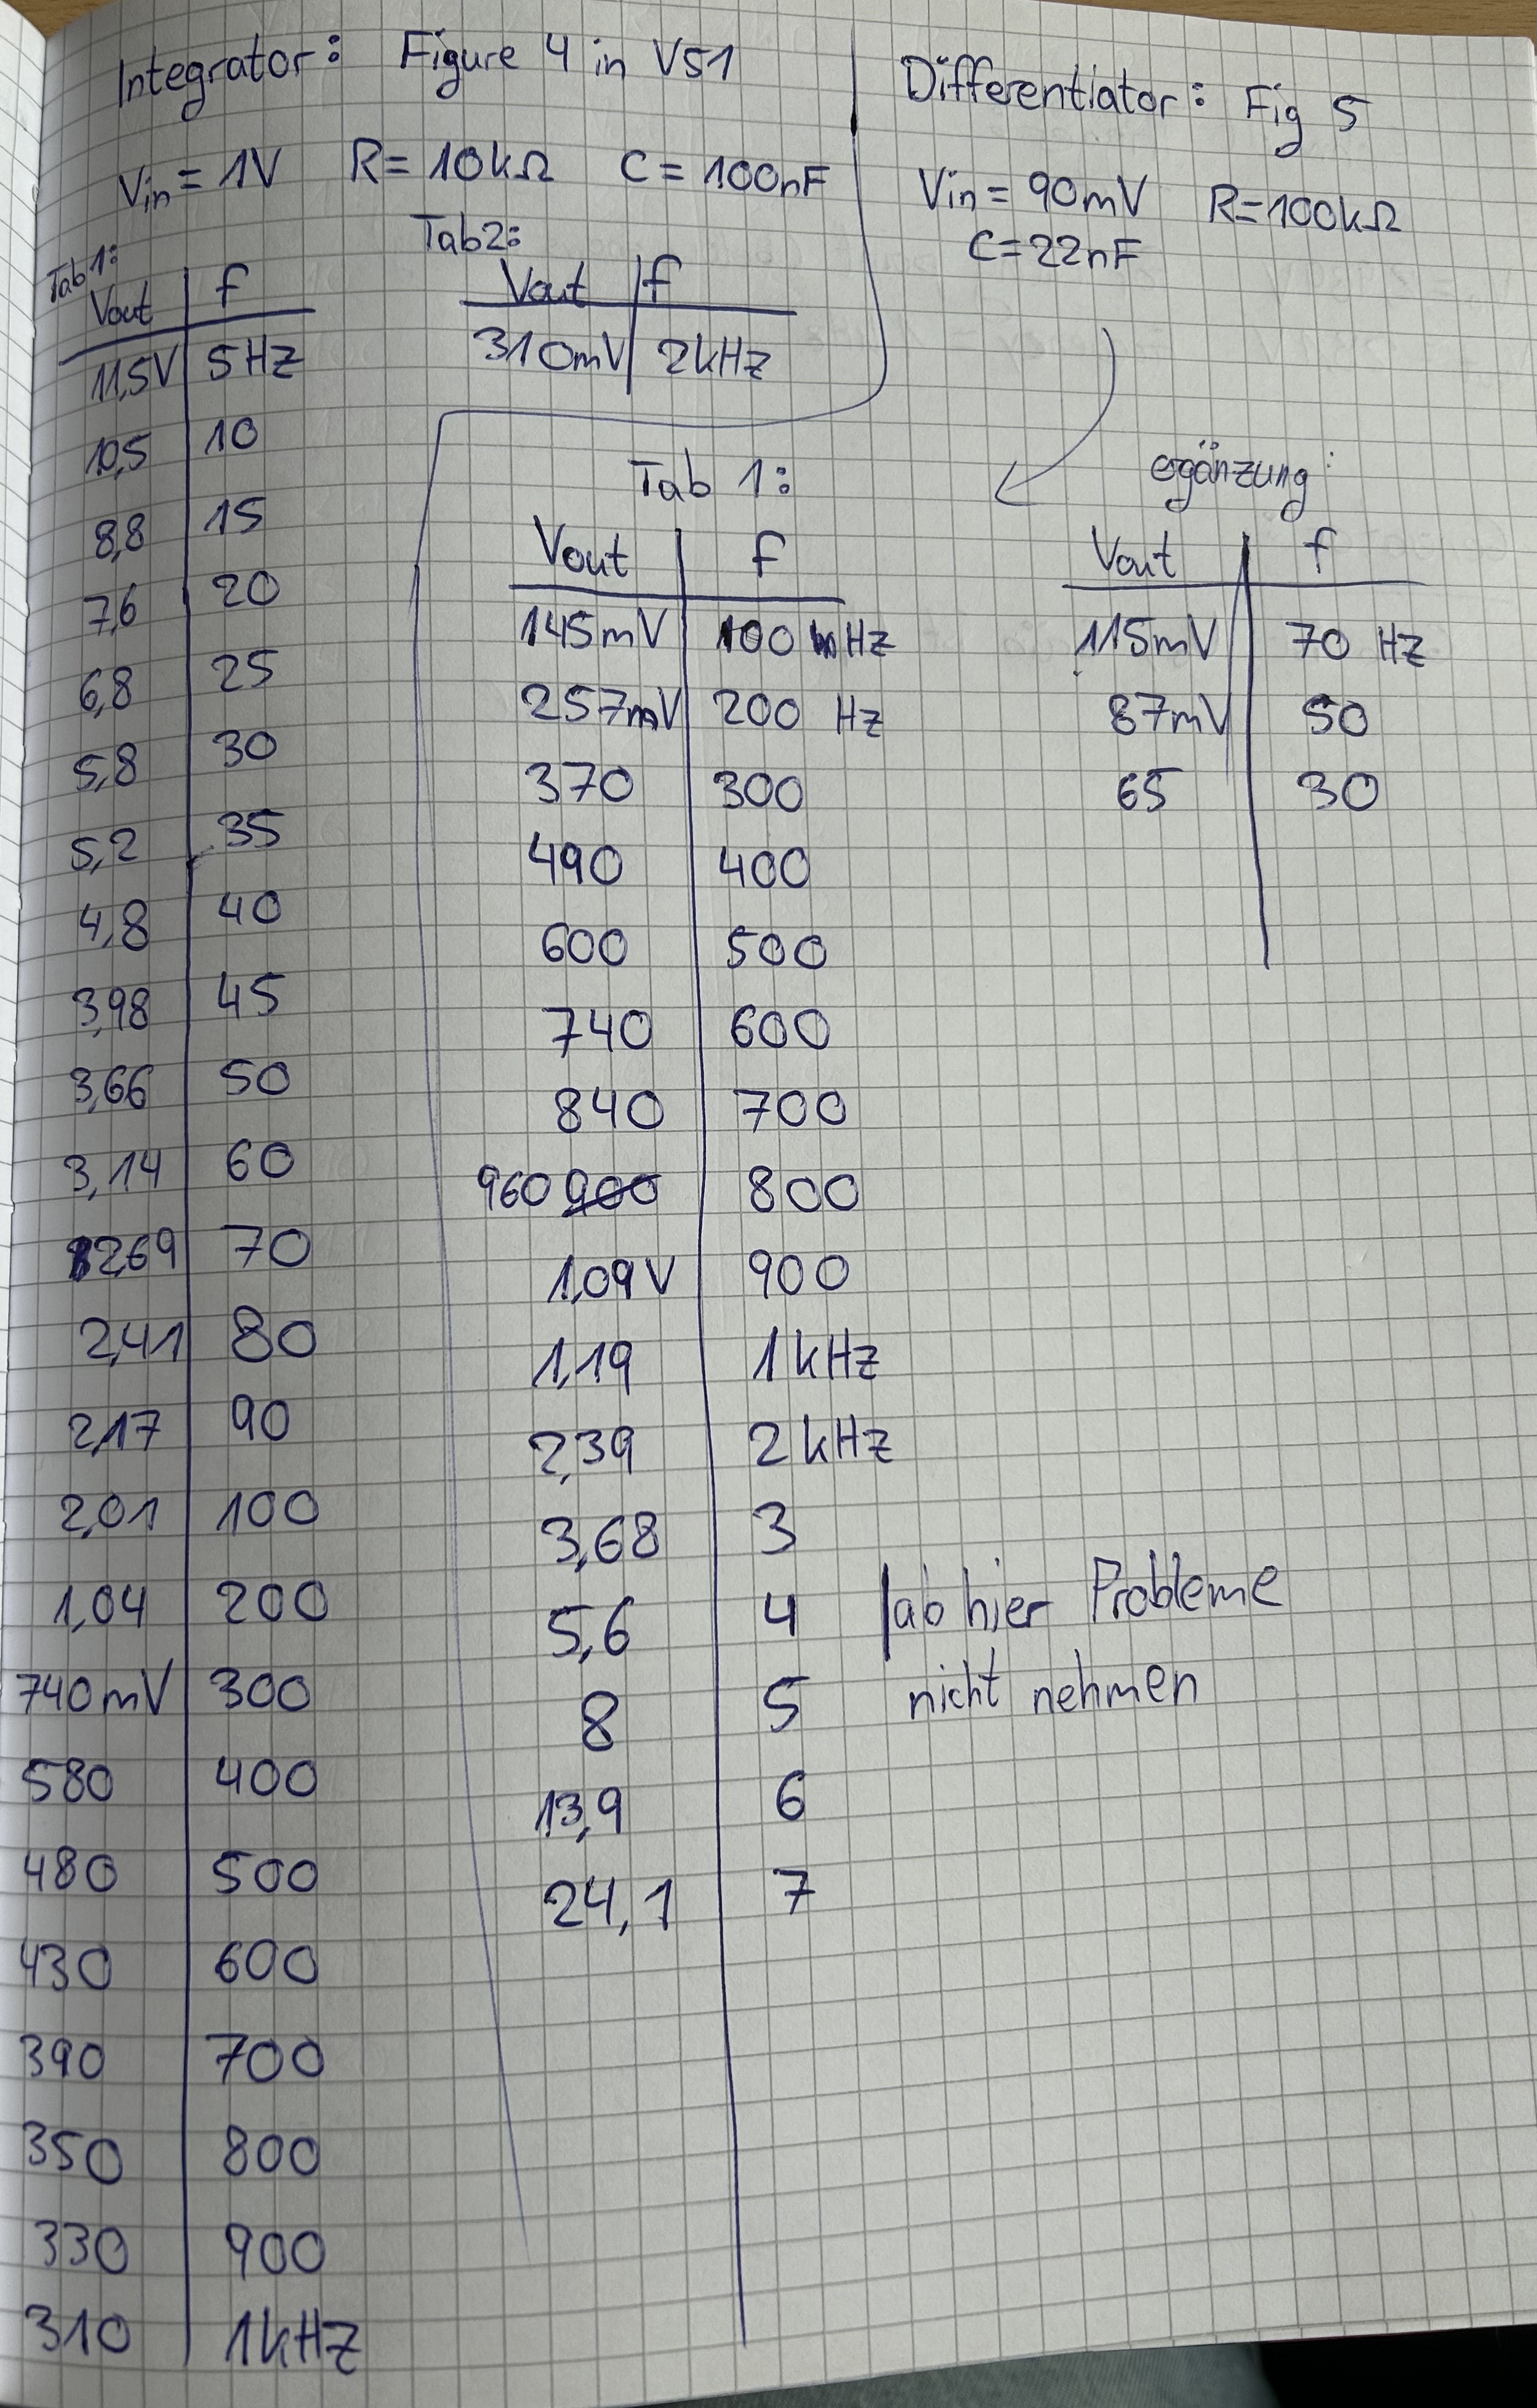
\includegraphics[width = 0.9\textwidth]{figures/Messdaten4.jpeg}
\end{figure}
\begin{figure}
  \centering
  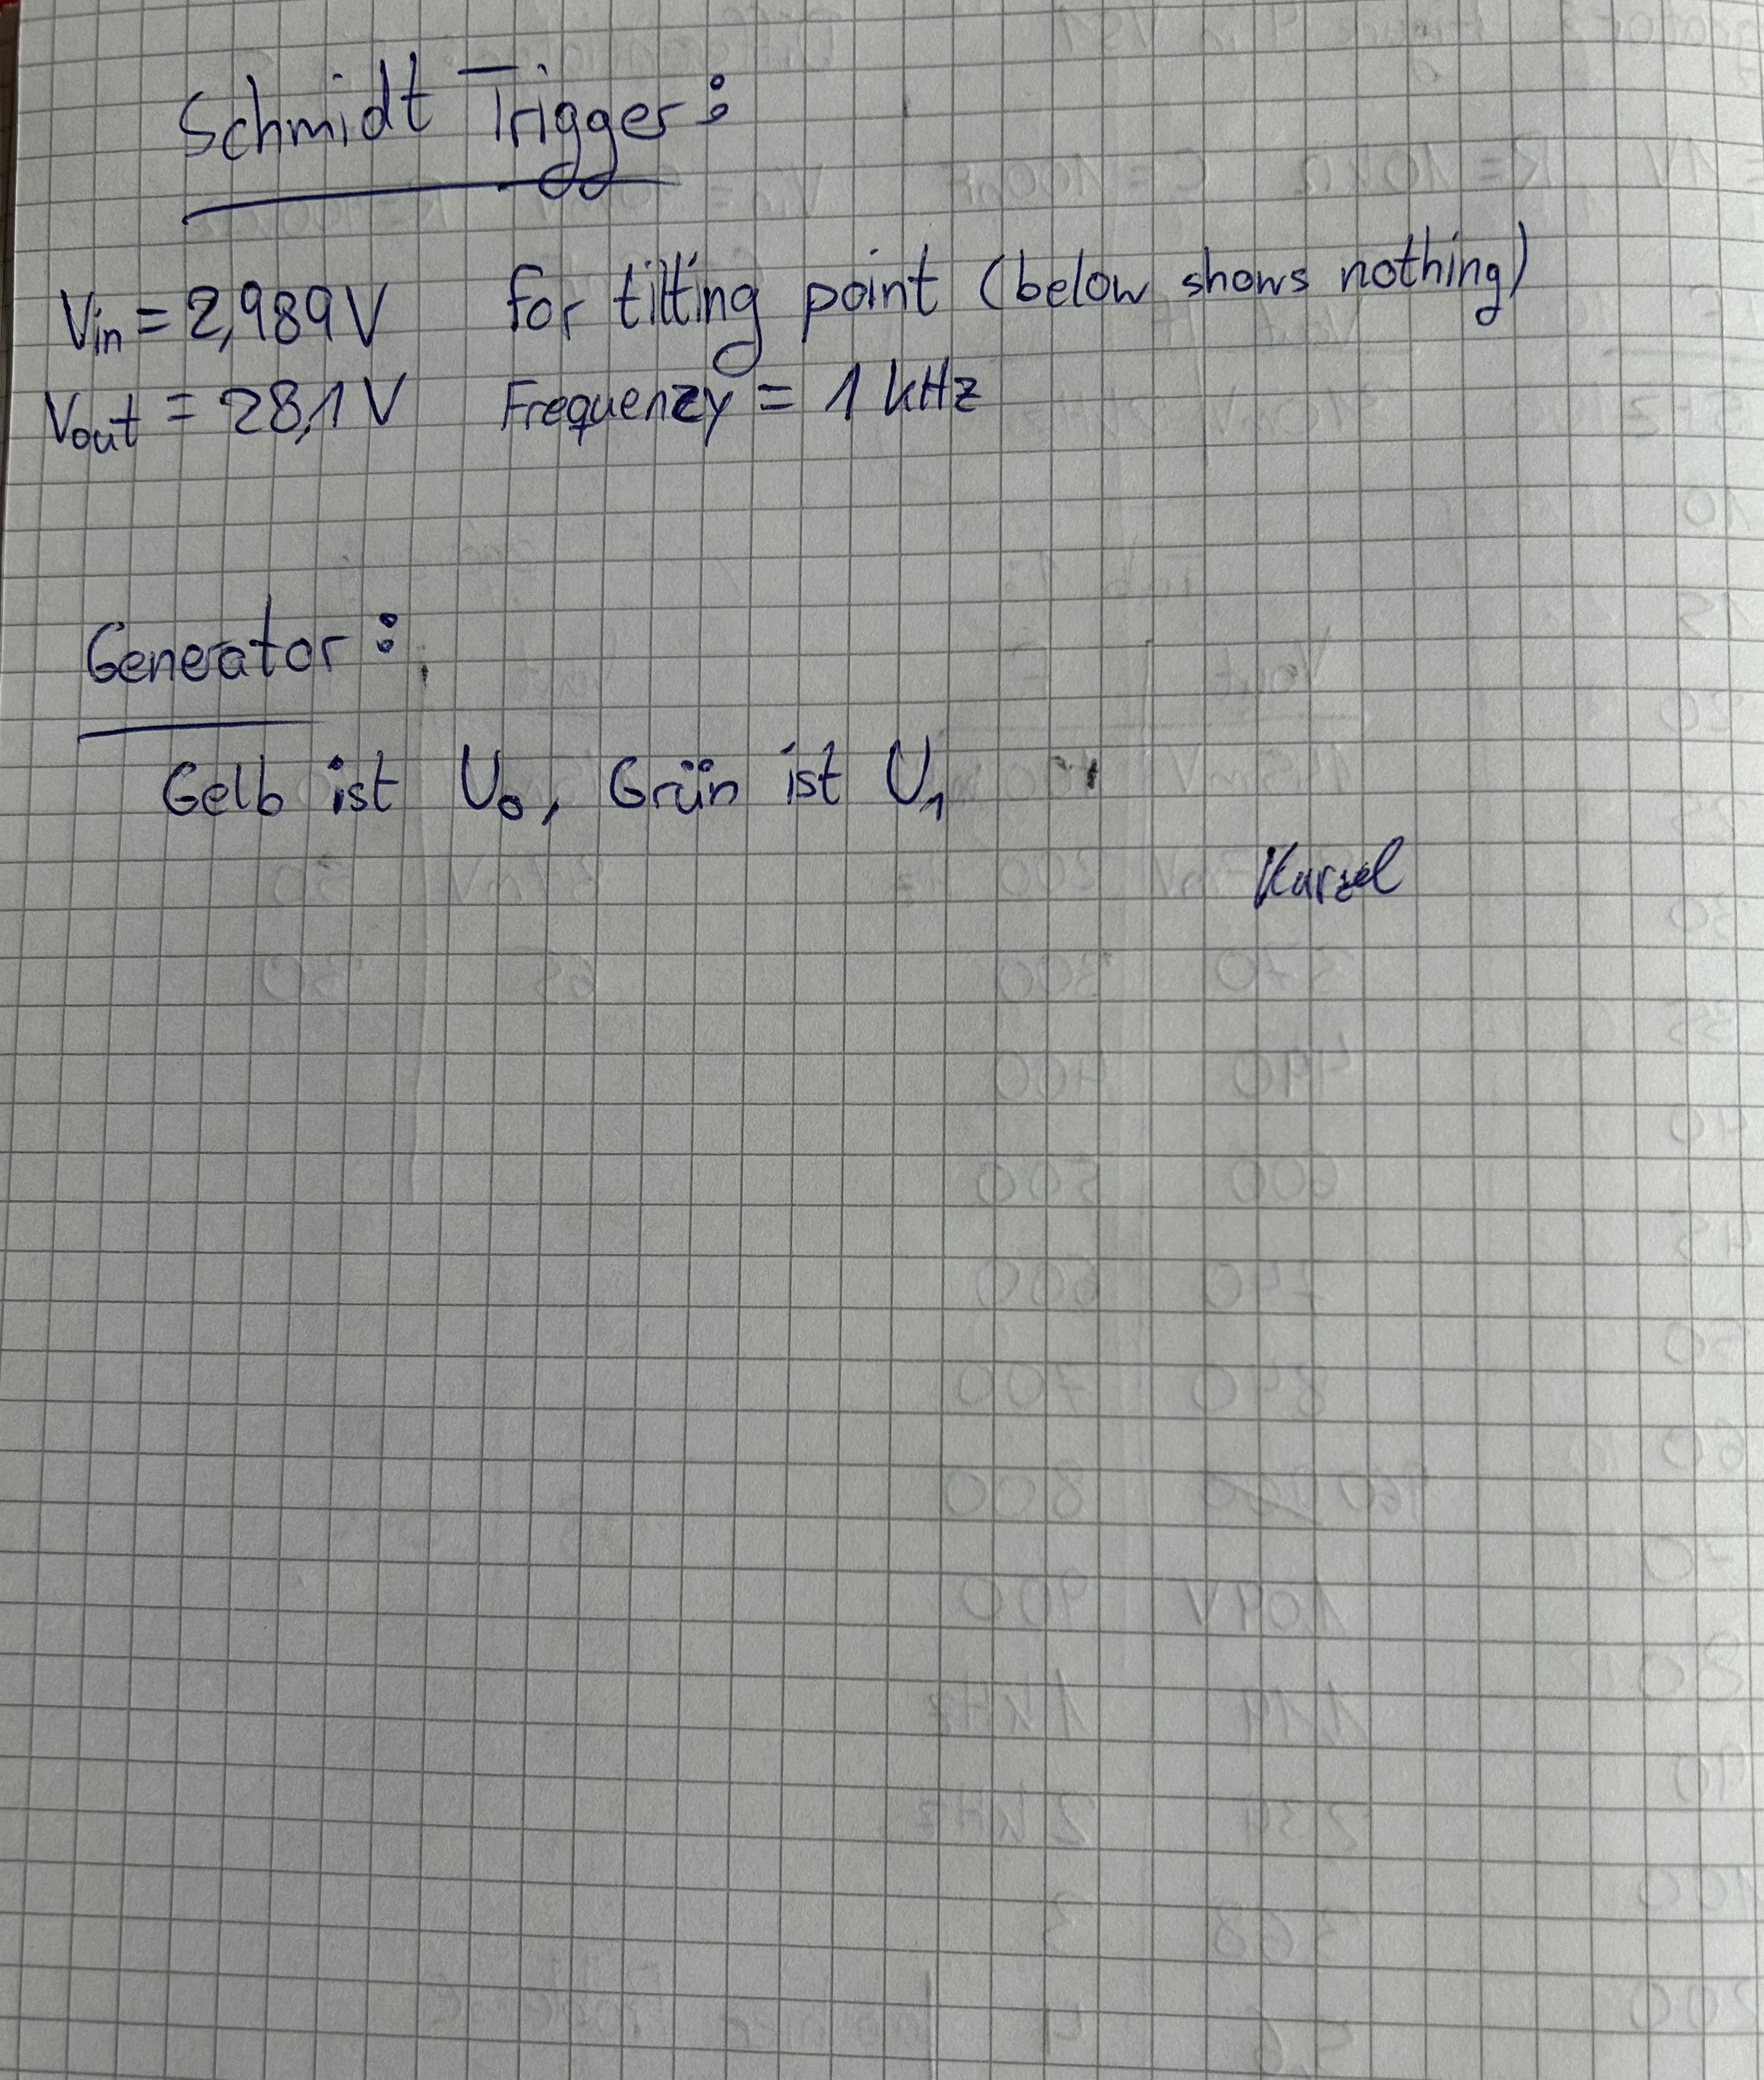
\includegraphics[width = 0.9\textwidth]{figures/Messdaten5.jpeg}
\end{figure}

\end{document}
